\documentclass[12pt,a4paper]{article}

% =========================================================================
% 1. CÁC GÓI CẦN THIẾT CHO BÁO CÁO MÔ PHỎNG / SYSTEMVERILOG
% =========================================================================
\usepackage[utf8]{inputenc}
\usepackage{parskip}
\setlength{\parskip}{0.8em}
\usepackage[vietnamese]{babel}
\usepackage[paperheight=29.7cm,paperwidth=21cm,right=2cm,left=2cm,top=2cm,bottom=2cm]{geometry}
\usepackage{amsmath,amssymb}
\usepackage{graphicx}
\usepackage{xcolor}
\usepackage{booktabs}
\usepackage{tabularx}
\usepackage{tikz}
\usetikzlibrary{calc}
\usepackage{fancyhdr}
\usepackage{hyperref}
\usepackage{listings}
\usepackage{float}

% =========================================================================
% 2. CẤU HÌNH HIỂN THỊ CODE SYSTEMVERILOG
% =========================================================================
\definecolor{sv_keyword}{rgb}{0.7, 0.1, 0.1}   % Đỏ đậm cho từ khóa
\definecolor{sv_type}{rgb}{0.1, 0.1, 0.8}      % Xanh dương cho kiểu dữ liệu
\definecolor{sv_comment}{rgb}{0.0, 0.5, 0.2}   % Xanh lá cho chú thích
\definecolor{sv_string}{rgb}{0.6, 0.1, 0.6}    % Tím cho chuỗi
\definecolor{sv_bg}{rgb}{0.97, 0.97, 0.97}

\lstdefinelanguage{SystemVerilog}{
    keywords=[1]{
        module, endmodule, input, output, logic, wire, reg, parameter, localparam,
        always_comb, always_ff, posedge, negedge, begin, end, if, else, case,
        endcase, default, typedef, enum, int, initial, assign
    },
    keywordstyle=[1]{\color{sv_keyword}\bfseries},
    keywords=[2]{state_t, clk, rst},
    keywordstyle=[2]{\color{sv_type}\bfseries},
    sensitive=true,
    morecomment=[l]{//},
    morecomment=[s]{/*}{*/},
    commentstyle=\color{sv_comment}\itshape,
    morestring=[b]",
    stringstyle=\color{sv_string}
}

\lstdefinestyle{sv_style}{
    language=SystemVerilog,
    backgroundcolor=\color{sv_bg},
    basicstyle=\ttfamily\footnotesize,
    numbers=left,
    numberstyle=\tiny\color{gray},
    numbersep=6pt,
    frame=single,
    rulecolor=\color{gray!40},
    breaklines=true,
    captionpos=b,
    keepspaces=true,
    tabsize=4
}
\lstset{style=sv_style}

% =========================================================================
% 3. CẤU HÌNH HEADER / FOOTER
% =========================================================================
\pagestyle{fancy}
\fancyhf{}
\setlength{\headheight}{15pt}
\fancyhead[L]{\small Project FPGA - Snake}
\fancyhead[R]{\small Báo cáo Mô phỏng \& Kiểm thử}
\renewcommand{\headrulewidth}{0.4pt}
\fancyfoot[R]{\small Trang \thepage}
\fancyfoot[L]{\small SVTH: Trần Hoàng An}
\renewcommand{\footrulewidth}{0.4pt}

\hypersetup{
    colorlinks=true,
    linkcolor=black,
    urlcolor=blue
}

\begin{document}

% =========================================================================
% TRANG BÌA (DÙNG NGUYÊN KHUNG VIỀN CŨ, CÂN ĐỐI LẠI BỐ CỤC)
% =========================================================================
\begin{titlepage}
    % Thuật toán vẽ viền đôi chuẩn Bách Khoa
    \begin{tikzpicture}[remember picture,overlay,inner sep=0,outer sep=0]
        \draw[blue!40!black,line width=4pt] 
            ([xshift=-1.8cm,yshift=-2.4cm]current page.north east) coordinate (A)--
            ([xshift=1.8cm,yshift=-2.4cm]current page.north west) coordinate(B)--
            ([xshift=1.8cm,yshift=2.4cm]current page.south west) coordinate (C)--
            ([xshift=-1.8cm,yshift=2.4cm]current page.south east) coordinate(D)--cycle;

        \draw ([yshift=0.5cm,xshift=-0.5cm]A)-- ([yshift=0.5cm,xshift=0.5cm]B)--
            ([yshift=-0.5cm,xshift=0.5cm]B) --([yshift=-0.5cm,xshift=-0.5cm]B)--
            ([yshift=0.5cm,xshift=-0.5cm]C)--([yshift=0.5cm,xshift=0.5cm]C)--
            ([yshift=-0.5cm,xshift=0.5cm]C)-- ([yshift=-0.5cm,xshift=-0.5cm]D)--
            ([yshift=0.5cm,xshift=-0.5cm]D)--([yshift=0.5cm,xshift=0.5cm]D)--
            ([yshift=-0.5cm,xshift=0.5cm]A)--([yshift=-0.5cm,xshift=-0.5cm]A)--
            ([yshift=0.5cm,xshift=-0.5cm]A);

        \draw ([yshift=-0.3cm,xshift=0.3cm]A)-- ([yshift=-0.3cm,xshift=-0.3cm]B)--
            ([yshift=0.3cm,xshift=-0.3cm]B) --([yshift=0.3cm,xshift=0.3cm]B)--
            ([yshift=-0.3cm,xshift=0.3cm]C)--([yshift=-0.3cm,xshift=-0.3cm]C)--
            ([yshift=0.3cm,xshift=-0.3cm]C)-- ([yshift=0.3cm,xshift=0.3cm]D)--
            ([yshift=-0.3cm,xshift=0.3cm]D)--([yshift=-0.3cm,xshift=-0.3cm]D)--
            ([yshift=0.3cm,xshift=-0.3cm]A)--([yshift=0.3cm,xshift=0.3cm]A)--
            ([yshift=-0.3cm,xshift=0.3cm]A);
    \end{tikzpicture}

    \begin{center}
        {\large\textbf{ĐẠI HỌC QUỐC GIA THÀNH PHỐ HỒ CHÍ MINH}}\\[0.15cm]
        {\large\textbf{TRƯỜNG ĐẠI HỌC BÁCH KHOA}}\\[0.15cm]
        {\large\textbf{KHOA ĐIỆN - ĐIỆN TỬ}}\\[0.1cm]
        {\rule{6cm}{0.6pt}}\\[0.8cm]

        % Logo to hơn (tăng từ 0.25 lên 0.35)
        
\includegraphics[width=0.35\textwidth]{images/logoBK.png}\\[1.0cm]

        % Cụm Tiêu đề chính cân đối
        {\fontsize{20pt}{23pt}\selectfont\textbf{BÁO CÁO MÔ PHỎNG VÀ KIỂM THỬ}}\\[0.4cm]
        {\fontsize{22pt}{26pt}\selectfont\textbf{THIẾT KẾ GAME SNAKE TRÊN FPGA}}\\[0.8cm]

        \vspace{0.5cm}
        % Thông tin Đề tài
        \parbox{1\textwidth}{
            \centering\fontsize{17pt}{23pt}\selectfont
            \textbf{Đề tài:} Thiết kế và kiểm thử hệ thống phần cứng trò chơi Snake\\
            điều khiển dải LED WS2812B trên kit FPGA Cyclone II
        }
    \end{center}

    \vfill

    % Khối Thông tin Sinh viên chi tiết, đầy đủ
    \begin{flushright}
        \parbox{0.68\textwidth}{
            \large
            \renewcommand{\arraystretch}{1.3}
            \begin{tabular}{ll}
                \textbf{Sinh viên thực hiện:} & Trần Hoàng An \\
                \textbf{MSSV:}                & 2410040 \\
                \textbf{Khóa / Lớp:}      & Khóa 24 / DD24ITN \\
                \textbf{Chuyên ngành:}        & Thiết kế Vi mạch (IC Design) \\
                \textbf{GitHub Repository:}   & \url{https://github.com/aokiii131}
            \end{tabular}
        }
        \hspace*{3.8cm}
    \end{flushright}

    \vspace{0.8cm}
    \begin{center}
        {\large Thành phố Hồ Chí Minh, tháng 09 năm 2026}
    \end{center}
    \vspace*{0.8cm}
\end{titlepage}

% =========================================================================
% MỤC LỤC
% =========================================================================
\newpage
\tableofcontents
\newpage

% =========================================================================
% NỘI DUNG CHÍNH
% =========================================================================
\section{Môi trường Kiểm thử \& Quy ước Thời gian}
\subsection{Công cụ Mô phỏng}
\begin{itemize}
    \item \textbf{Phần mềm mô phỏng:} QuestaSim 23.1
    \item \textbf{Ngôn ngữ thiết kế \& kiểm thử:} SystemVerilog (IEEE 1800-2012)
    \item \textbf{FPGA Target:} Altera Cyclone II (Kit DE2)
\end{itemize}

\subsection{Quy ước Xung nhịp và Đơn vị Thời gian}
\begin{itemize}
    \item Xung nhịp hệ thống ($clk$): $50\text{ MHz} \implies T_{clk} = 20\text{ ns}$.
    \item Độ phân giải thời gian mô phỏng: \texttt{timescale 1ns/1ps}.
\end{itemize}

\newpage

% =========================================================================
% PHẦN 2: MÔ PHỎNG CHI TIẾT MODULE WS2812B DRIVER
% =========================================================================
\section{Kết quả Mô phỏng Module WS2812B Driver}

\subsection{Mục tiêu Kiểm thử và Cấu hình Testbench}

Module \texttt{ws2812b\_driver} đảm nhiệm việc chốt dữ liệu hình ảnh logic từ Game Engine và điều chế thành chuỗi xung số NZR đơn dây theo đúng chuẩn thời gian của chip WS2812B.

Để tối ưu hóa thời gian chạy mô phỏng trên ModelSim/QuestaSim (tránh phải chờ hàng triệu chu kỳ xung nhịp cho 60 LED và $300\,\mu\text{s}$ Latch), môi trường Testbench (\texttt{ws2812b\_driver\_tb}) đã override các tham số phần cứng thông qua cơ chế Parameterization:
\begin{itemize}
    \item \texttt{LED\_COUNT = TEST\_LEDS = 3} (Kiểm thử rút gọn trên 3 LED thay vì 60 LED).
    \item \texttt{RES = TEST\_RES = 50} (Rút ngắn thời gian chốt khung hình xuống 50 chu kỳ clock thay vì 15,000 chu kỳ).
    \item Chu kỳ Master Clock: $T_{clk} = 20\text{ ns}$ ($50\text{ MHz}$).
    \item Tham số định thời bit chuẩn: $T_{0H} = 15\text{ ck}$ ($300\text{ ns}$), $T_{0L} = 40\text{ ck}$ ($800\text{ ns}$), $T_{1H} = 40\text{ ck}$ ($800\text{ ns}$), $T_{1L} = 15\text{ ck}$ ($300\text{ ns}$). Tổng chu kỳ mỗi bit là $55\text{ ck}$ ($1100\text{ ns}$).
\end{itemize}

\subsection{Kế hoạch Kiểm thử Toàn diện (Verification Test Plan)}
Kế hoạch kiểm thử của module bao gồm 7 kịch bản kiểm tra toàn diện hoạt động của mạch, từ phản hồi mức thanh ghi, định thời dạng sóng PWM, chuyển trạng thái biên cho tới tính độc lập của bộ đệm khung hình:
\begin{enumerate}
    \item \textbf{TC01 - Reset Behavior:} Kiểm tra tín hiệu \texttt{rst} khởi tạo thành công FSM về trạng thái \texttt{LOAD}, các thanh ghi đếm được đặt về giá trị mặc định (\texttt{pixel\_counter = 0}, \texttt{bit\_counter = 23}, \texttt{timing\_counter = 0}) và ngõ ra \texttt{led\_data\_out} giữ mức logic 0.
    \item \textbf{TC02 - Frame Capturing (LOAD):} Kiểm tra khả năng chốt dữ liệu mảng từ cổng \texttt{pixel\_data} vào bộ đệm nội bộ \texttt{tx\_frame} trong chu kỳ \texttt{LOAD} bằng kích thích ngẫu nhiên có ràng buộc \texttt{\$urandom\_range(4, 0)}.
    \item \textbf{TC03 - Serialization Traversal (SEND):} Kiểm tra quy trình tuần tự hóa dữ liệu khi phát khung: duyệt tuần tự pixel từ $0 \to 2$ (\texttt{TEST\_LEDS = 3}) và truyền bit theo thứ tự MSB-first từ $23 \to 0$ cho từng pixel.
    \item \textbf{TC04 - Bit Waveform Timing:} Kiểm tra độ chính xác xung PWM trên ngõ ra \texttt{led\_data\_out} theo chuẩn WS2812B: Bit 0 ($15\text{ ck HIGH} / 40\text{ ck LOW}$) và Bit 1 ($40\text{ ck HIGH} / 15\text{ ck LOW}$), tổng chu kỳ mỗi bit đạt chính xác $55\text{ ck}$ ($1100\text{ ns}$).
    \item \textbf{TC05 - Boundary Transition (SEND $\to$ LATCH):} Xác nhận điều kiện biên tại thời điểm kết thúc khung hình (\texttt{pixel\_counter = 2}, \texttt{bit\_counter = 0}, \texttt{timing\_counter = 54}), FSM chuyển chính xác sang trạng thái \texttt{LATCH}.
    \item \textbf{TC06 - Frame Latch Integrity:} Kiểm tra trong suốt trạng thái \texttt{LATCH}, ngõ ra \texttt{led\_data\_out} luôn giữ mức LOW tuyệt đối đủ $50\text{ chu kỳ}$ ($1000\text{ ns}$ theo \texttt{TEST\_RES = 50}) trước khi FSM tự động quay về \texttt{LOAD}.
    \item \textbf{TC07 - Frame Snapshot Isolation:} Kiểm tra tính cô lập khung truyền: thay đổi đột ngột giá trị \texttt{pixel\_data} sang \texttt{\{3'b010, 3'b011, 3'b000\}} ngay khi FSM đang ở trạng thái \texttt{SEND}, đảm bảo bộ đệm \texttt{tx\_frame} và bus giải mã 24-bit không bị biến động.
\end{enumerate}

\subsection{Bảng Tổng hợp Trạng thái Kiểm thử}
\begin{table}[H]
    \centering
    \caption{Bảng tổng hợp kết quả thực thi các Test Cases của WS2812B Driver}
    \label{tab:driver_test_cases}
    \begin{tabularx}{\textwidth}{c p{3.2cm} p{7.5cm} >{\centering\arraybackslash}X}
        \toprule
        \textbf{STT} & \textbf{Kịch bản} & \textbf{Tiêu chí Đánh giá} & \textbf{Kết quả} \\
        \midrule
        TEST CASE 1 & Reset Behavior & FSM vào \texttt{LOAD}, các bộ đếm reset về 0, \texttt{led\_data\_out} = 0 & \textcolor{teal}{\textbf{PASS}} \\
        TEST CASE 2 & TX Frame Capture & Dữ liệu \texttt{tx\_frame} khớp 100\% với \texttt{pixel\_data} & \textcolor{teal}{\textbf{PASS}} \\
        TEST CASE 3 & Sending Completion & Quét tuần tự pixel $0 \to 2$, bit $23 \to 0$ và hoàn tất phát chuyển sang \texttt{LATCH} & \textcolor{teal}{\textbf{PASS}} \\
        TEST CASE 4 & Latching Completion & Giữ mức LOW đủ 50 ck ($1\,\mu\text{s}$) và hoàn tất chốt để quay về \texttt{LOAD} & \textcolor{teal}{\textbf{PASS}} \\
        TEST CASE 5 & Snapshot Isolation & Đổi \texttt{pixel\_data} giữa lúc \texttt{SEND} không làm biến đổi \texttt{tx\_frame} đang phát & \textcolor{teal}{\textbf{PASS}} \\
        \bottomrule
    \end{tabularx}
\end{table}

\subsection{Bằng chứng Mô phỏng Thực tế (Waveform Evidence)}

\subsubsection{Test Case 01: Hành vi Khởi tạo và Reset (Reset Behavior)}
\begin{itemize}
    \item \textbf{Điều kiện kích thích:} Tác động xung \texttt{rst = 1} trong 2 chu kỳ xung nhịp, sau đó hạ về 0 tại cạnh âm của xung nhịp.
    \item \textbf{Kết quả mô phỏng:} 
    \begin{itemize}
        \item FSM khởi tạo tức thì vào trạng thái \texttt{LOAD} .
        \item Các biến đếm \texttt{pixel\_counter = 0}, \texttt{bit\_counter = 23}, và \texttt{timing\_counter = 0}.
        \item Tín hiệu \texttt{led\_data\_out} giữ mức logic 0, không xuất hiện bất kỳ xung nhiễu nào.
    \end{itemize}
\end{itemize}

\begin{figure}[htbp]
    \centering
    % Khi có ảnh thật, thay khung \fbox bằng lệnh: 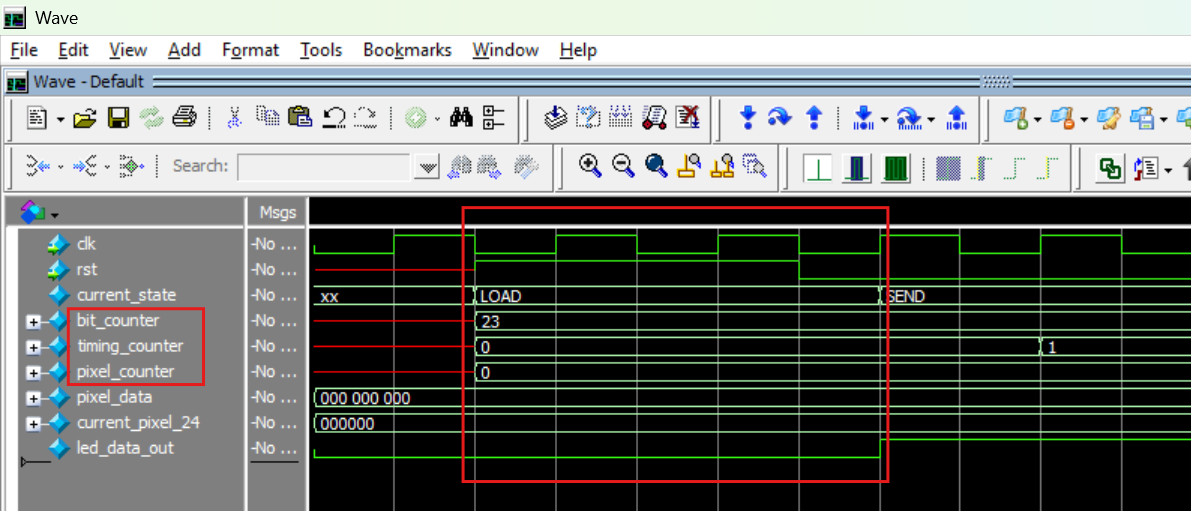
\includegraphics[width=0.9\textwidth]{images/wf_tc01_reset.png}
    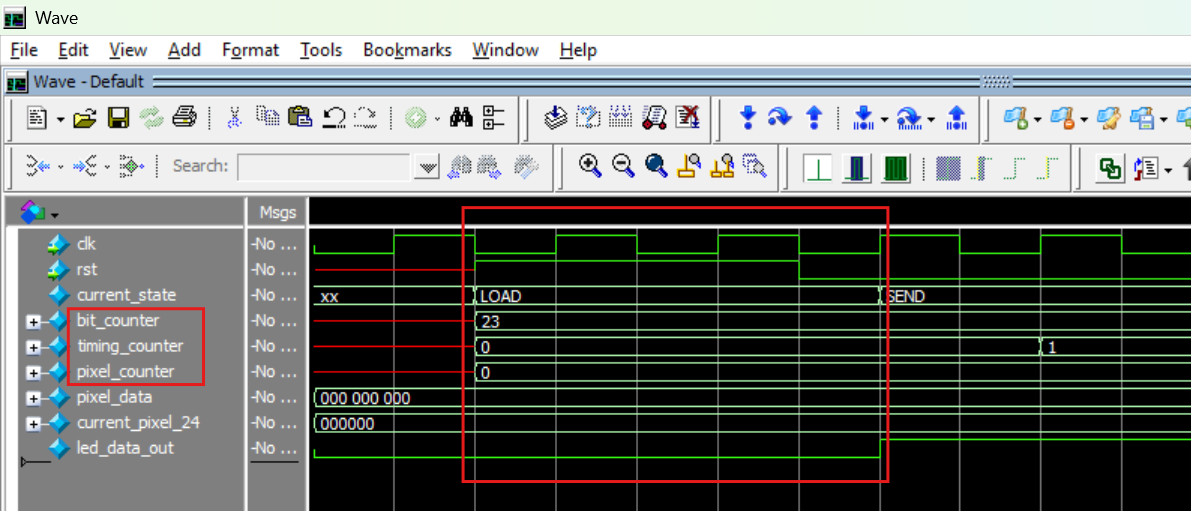
\includegraphics[width=0.9\textwidth]{images/wf_tc01_reset.png}    
    \caption{Dạng sóng kiểm tra hành vi Reset của module Driver}
    \label{fig:wf_tc01}
\end{figure}

\subsubsection{Test Case 02: Nạp Khung hình vào Bộ đệm (TX Frame Capture)}
\begin{itemize}
    \item \textbf{Điều kiện kích thích:} Sinh ngẫu nhiên giá trị màu cho 3 pixel thông qua hàm \texttt{\$urandom\_range(4,0)}. Quan sát sự tương quan giữa mảng đầu vào \texttt{pixel\_data} và mảng thanh ghi nội bộ \texttt{tx\_frame}.
    \item \textbf{Kết quả Console log:} Toàn bộ giá trị từ \texttt{pixel\_data[0..2]} được sao chép nguyên vẹn sang \texttt{tx\_frame[0..2]} ngay khi FSM trải qua trạng thái \texttt{LOAD}:
\end{itemize}

\begin{figure}[htbp]
    \centering
    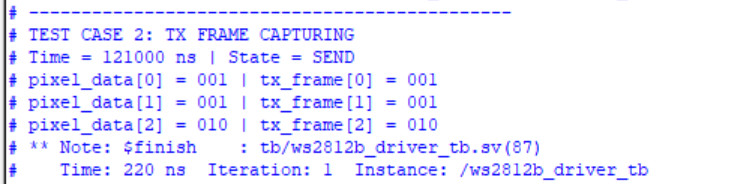
\includegraphics[width=0.9\textwidth]{images/cs_tc02_capture.png}
    \caption{Console Log ghi nhận dữ liệu nạp vào tx\_frame từ pixel\_data}
    \label{fig:cs_tc02}
\end{figure}

    \begin{figure}[htbp]
    \centering
    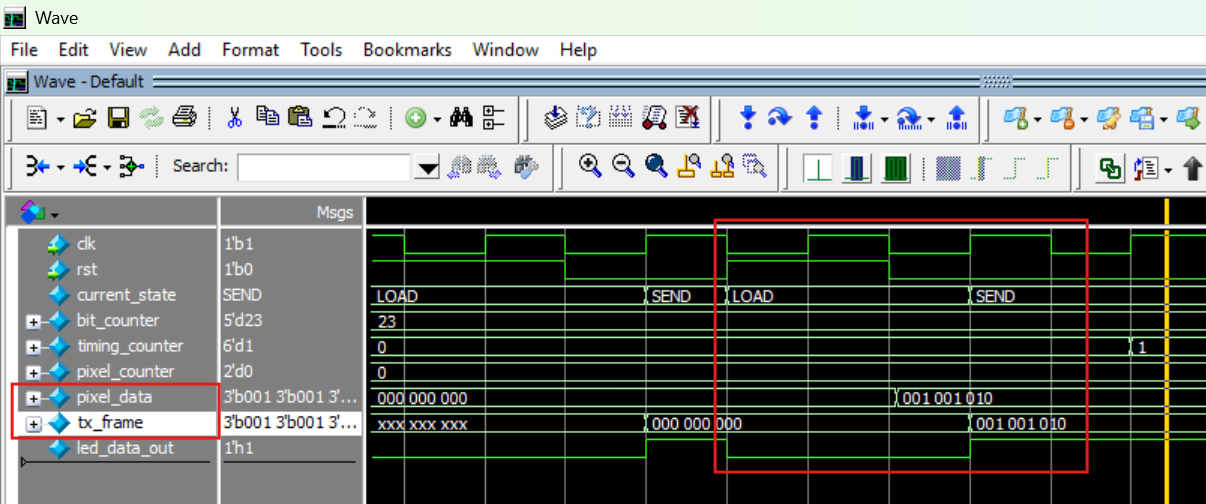
\includegraphics[width=0.9\textwidth]{images/wf_tc02_capture.png}
    \caption{Dữ liệu hình ảnh được chốt an toàn vào thanh ghi truyền dẫn}
    \label{fig:wf_tc02}
\end{figure}

\subsubsection{Test Case 03: Quét Tuần tự Pixel và Bit (Serialization Traversal)}
\begin{itemize}
    \item \textbf{Điều kiện kích thích:} Quan sát tiến trình vận hành của FSM khi duy trì ở trạng thái \texttt{SEND}.
    \item \textbf{Phân tích dạng sóng:} 
    \begin{itemize}
        \item Bộ đếm \texttt{bit\_counter} thực hiện đếm lùi chính xác từ 23 về 0 cho mỗi gói dữ liệu pixel.
        \item Ngay tại chu kỳ \texttt{bit\_counter} đạt giá trị 0 và hoàn tất 55 chu kỳ truyền, \texttt{pixel\_counter} tự động tăng thêm 1 đơn vị (từ 0 lên 1) đồng thời \texttt{bit\_counter} lập tức nạp lại giá trị 23 để bắt đầu truyền pixel tiếp theo. 
        \item Cơ chế này đảm bảo toàn bộ khung hình được tuần tự hóa liên tục theo đúng chuẩn MSB-first mà không bị mất nhịp.
    \end{itemize}
\end{itemize}

\begin{figure}[H]
    \centering
    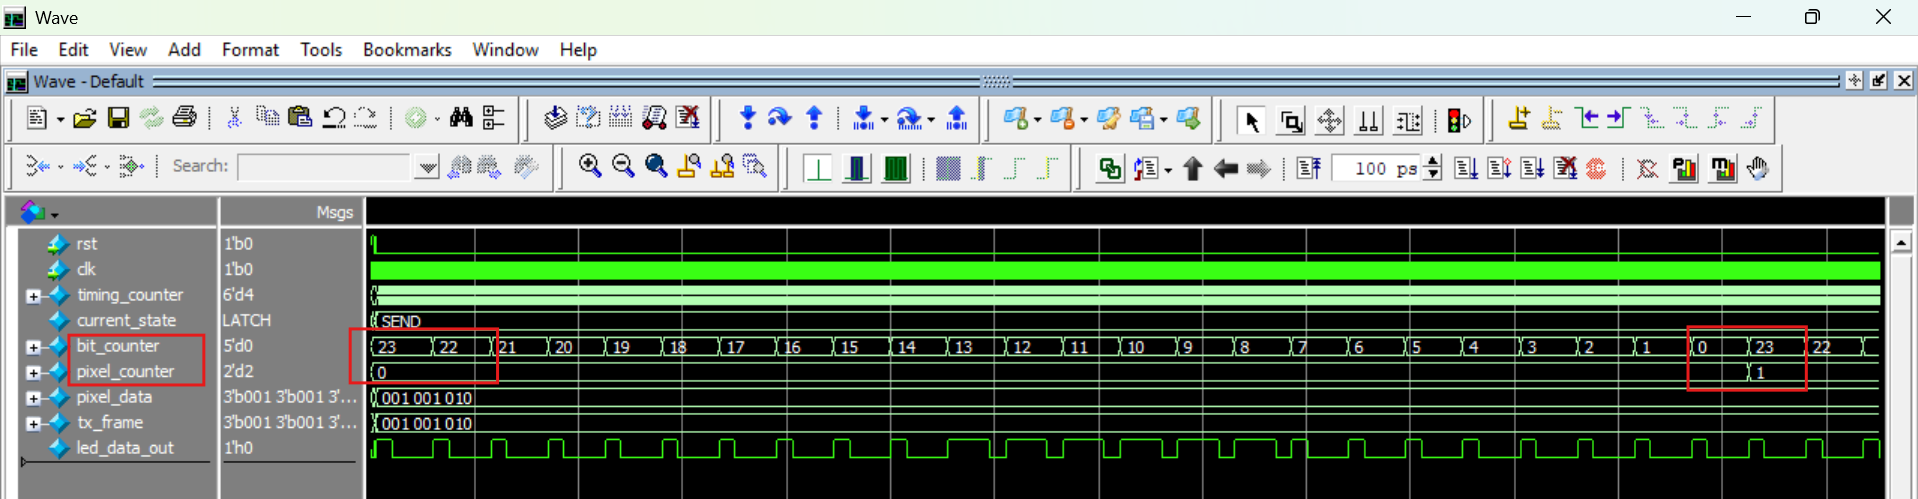
\includegraphics[width=\textwidth]{images/wf_tc03_sending.png}
    \caption{Dạng sóng tiến trình quét tuần tự Pixel và Bit trong trạng thái SEND}
    \label{fig:wf_tc03_sending}
\end{figure}

\subsubsection{Test Case 04: Độ chính xác Dạng sóng PWM (Bit Waveform Timing)}
\begin{itemize}
    \item \textbf{Điều kiện kích thích:} Sử dụng công cụ đo lường (Cursor) trên ModelSim để xác minh độ rộng xung HIGH và LOW của tín hiệu ngõ ra \texttt{led\_data\_out} khi phát bit 1 và bit 0.
    \item \textbf{Kết quả đo đạc:}
    \begin{itemize}
        \item \textbf{Mã hóa Bit 1:} Quan sát tại thời điểm \texttt{bit\_counter = 12}, tín hiệu \texttt{current\_bit} nhận giá trị \texttt{1} từ bus \texttt{current\_pixel\_24}. Dạng sóng ngõ ra \texttt{led\_data\_out} ghi nhận mức HIGH xấp xỉ 800 ns ($T_{1H}$) và mức LOW xấp xỉ 300 ns ($T_{1L}$). Tổng thời lượng đạt chính xác 55 chu kỳ ($1100\text{ ns}$).
        \item \textbf{Mã hóa Bit 0:} Khi \texttt{current\_bit} mang giá trị \texttt{0}, tín hiệu duy trì mức HIGH trong 15 chu kỳ xung nhịp ($300\text{ ns}$) và mức LOW trong 40 chu kỳ ($800\text{ ns}$). Tổng thời lượng đạt chính xác 55 chu kỳ ($1100\text{ ns}$).
    \end{itemize}
\end{itemize}

\begin{figure}[H]
    \centering
    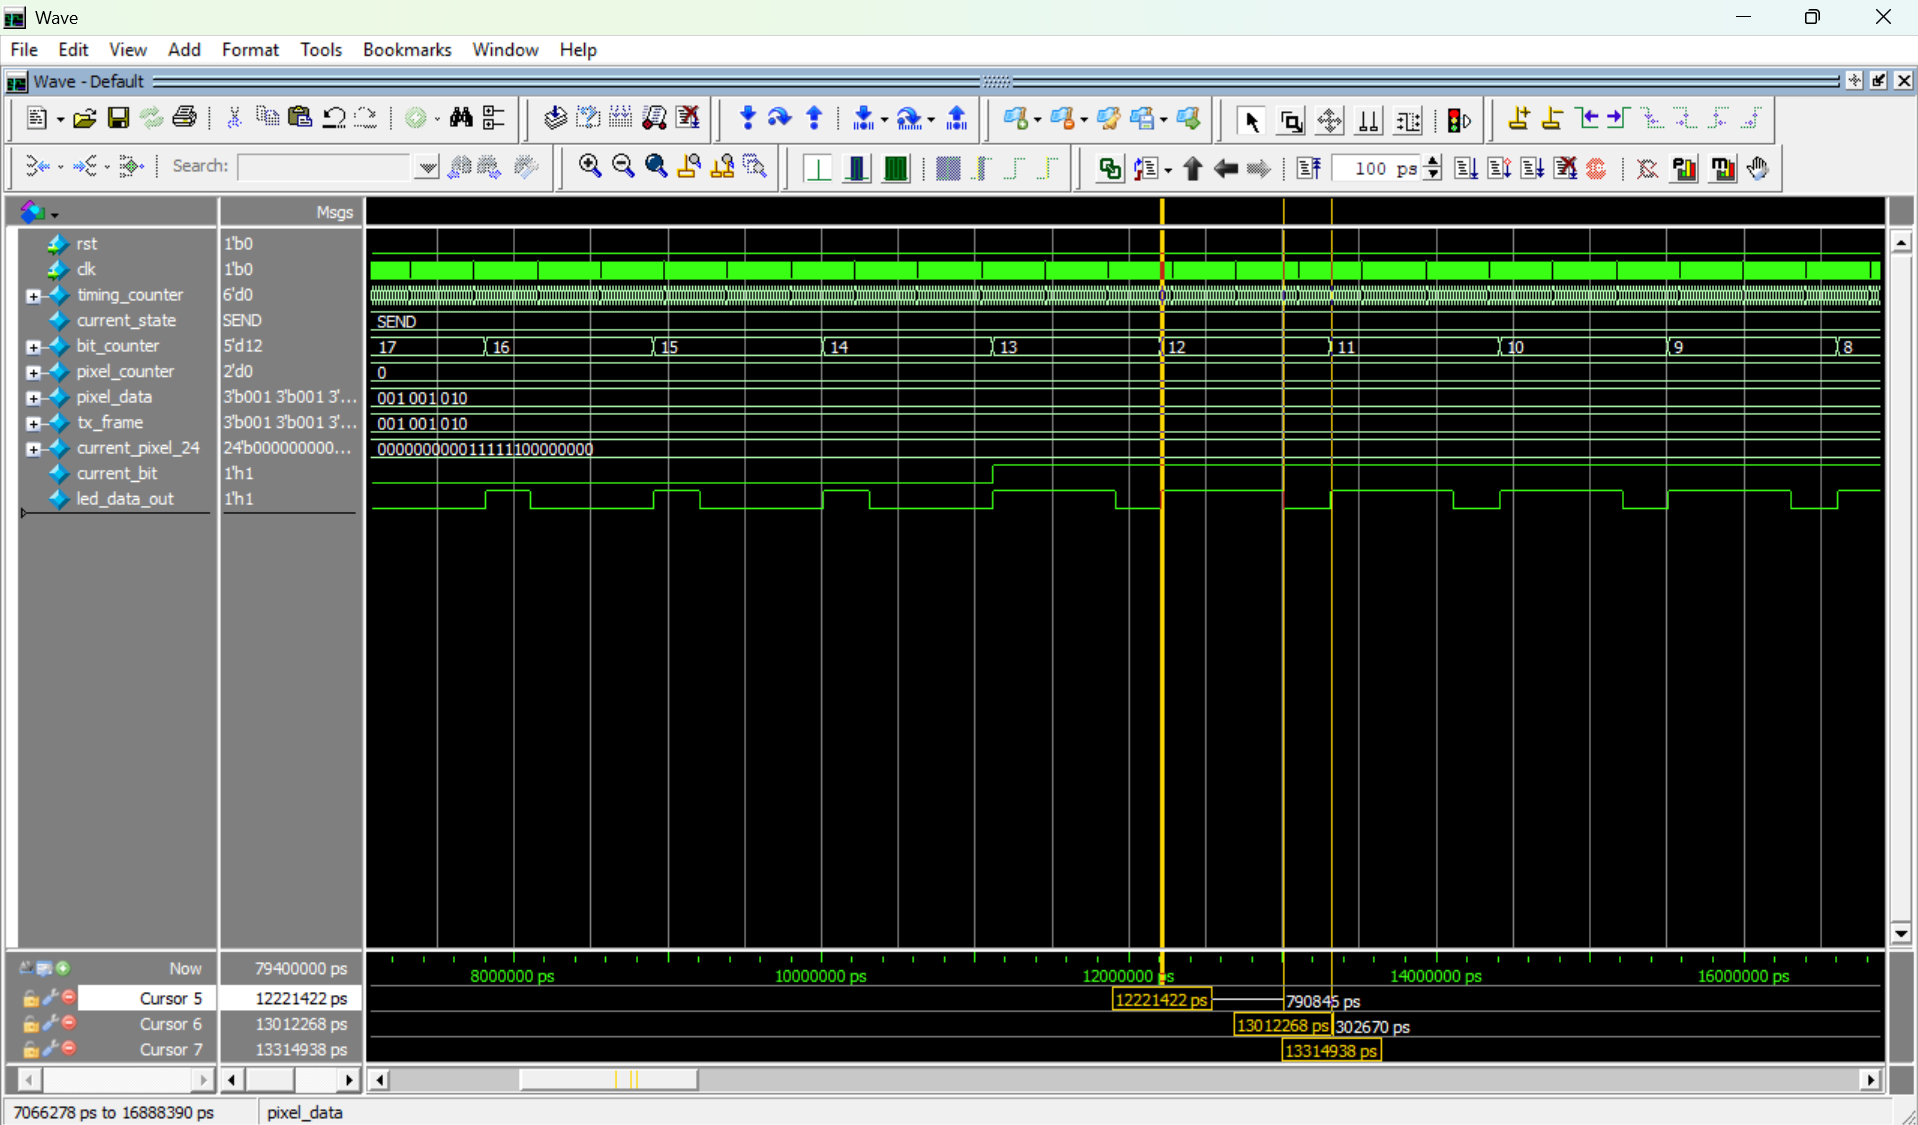
\includegraphics[width=\textwidth]{images/wf_tc4_bit1.png} 
    \caption{Phân tích độ rộng xung PWM khi truyền Bit 1 (tại bit\_counter = 12)}
    \label{fig:wf_tc04_timing_bit1}
\end{figure}

\begin{figure}[H]
    \centering
    % CHÚ Ý: Chèn ảnh phân tích độ rộng xung cho Bit 0 vào đường dẫn này
    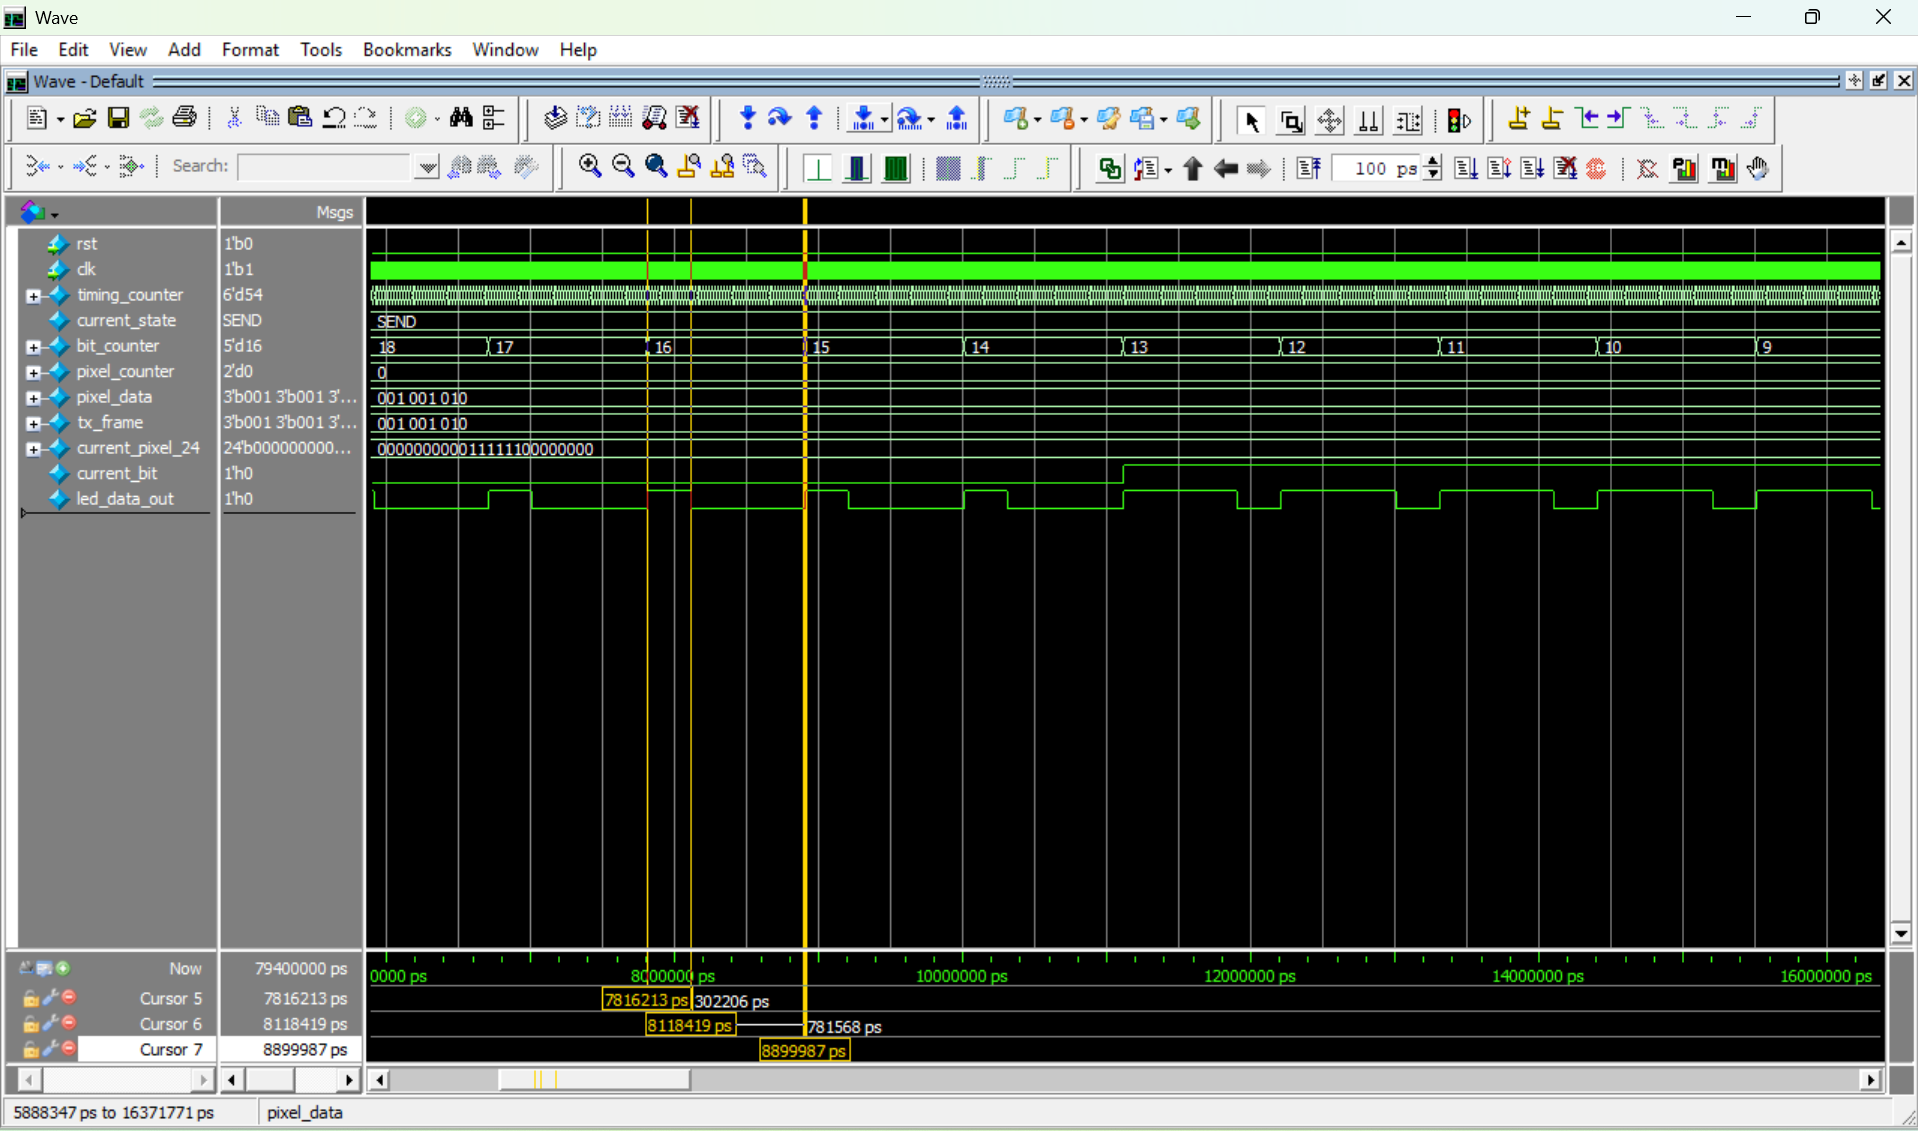
\includegraphics[width=\textwidth]{images/wf_tc4_bit0.png} 
    \caption{Phân tích độ rộng xung PWM khi truyền Bit 0}
    \label{fig:wf_tc04_timing_bit0}
\end{figure}


\subsubsection{Test Case 05 \& 06: Chuyển Trạng thái Biên và Thời gian Chốt Khung (Boundary Transition \& Latch Verification)}
\begin{itemize}
    \item \textbf{Điều kiện kích thích:} Quan sát thời điểm hoàn tất truyền bit cuối cùng của pixel cuối cùng trong khung hình (\texttt{pixel\_counter = 2}, \texttt{bit\_counter = 0}) và tiến trình thực thi trạng thái \texttt{LATCH}.
    \item \textbf{Phân tích dạng sóng:}
    \begin{itemize}
        \item \textbf{Chuyển trạng thái biên (Boundary Transition):} Đúng tại thời điểm \texttt{pixel\_counter = 2} (pixel thứ 3 theo tham số \texttt{TEST\_LEDS = 3}) và \texttt{bit\_counter = 0} kết thúc 55 chu kỳ truyền xung, FSM chuyển trạng thái từ \texttt{SEND} sang \texttt{LATCH} tại vị trí vạch đo Cursor 9 ($79.308\,\mu\text{s}$). Sau đó, khi RES hết, FSM tự động quay về trạng thái \texttt{LOAD} tại vạch đo Cursor 10 ($80.330\,\mu\text{s}$).
        \item \textbf{Tính toàn vẹn thời gian Latch (Latch Integrity):} Trong suốt trạng thái \texttt{LATCH}, đường tín hiệu ngõ ra \texttt{led\_data\_out} được giữ ở mức 0 tuyệt đối. 
        \item \textbf{Đo kiểm chu kỳ trễ RES:} Theo cấu hình Testbench với \texttt{TEST\_RES = 50}, thời gian lý thuyết giữ mức LOW là $50 \times 20\text{ ns} = 1000\text{ ns}$ ($1.0\,\mu\text{s}$). Kết quả đo thực tế giữa Cursor 9 và Cursor 10 đạt xấp xỉ $1021971\text{ ps} \approx 1022\text{ ns}$ ($\approx 1.02\,\mu\text{s}$), hoàn toàn khớp với chu kỳ thiết kế trước khi hệ thống kết thúc khung truyền.
    \end{itemize}
\end{itemize}

\begin{figure}[H]
    \centering
    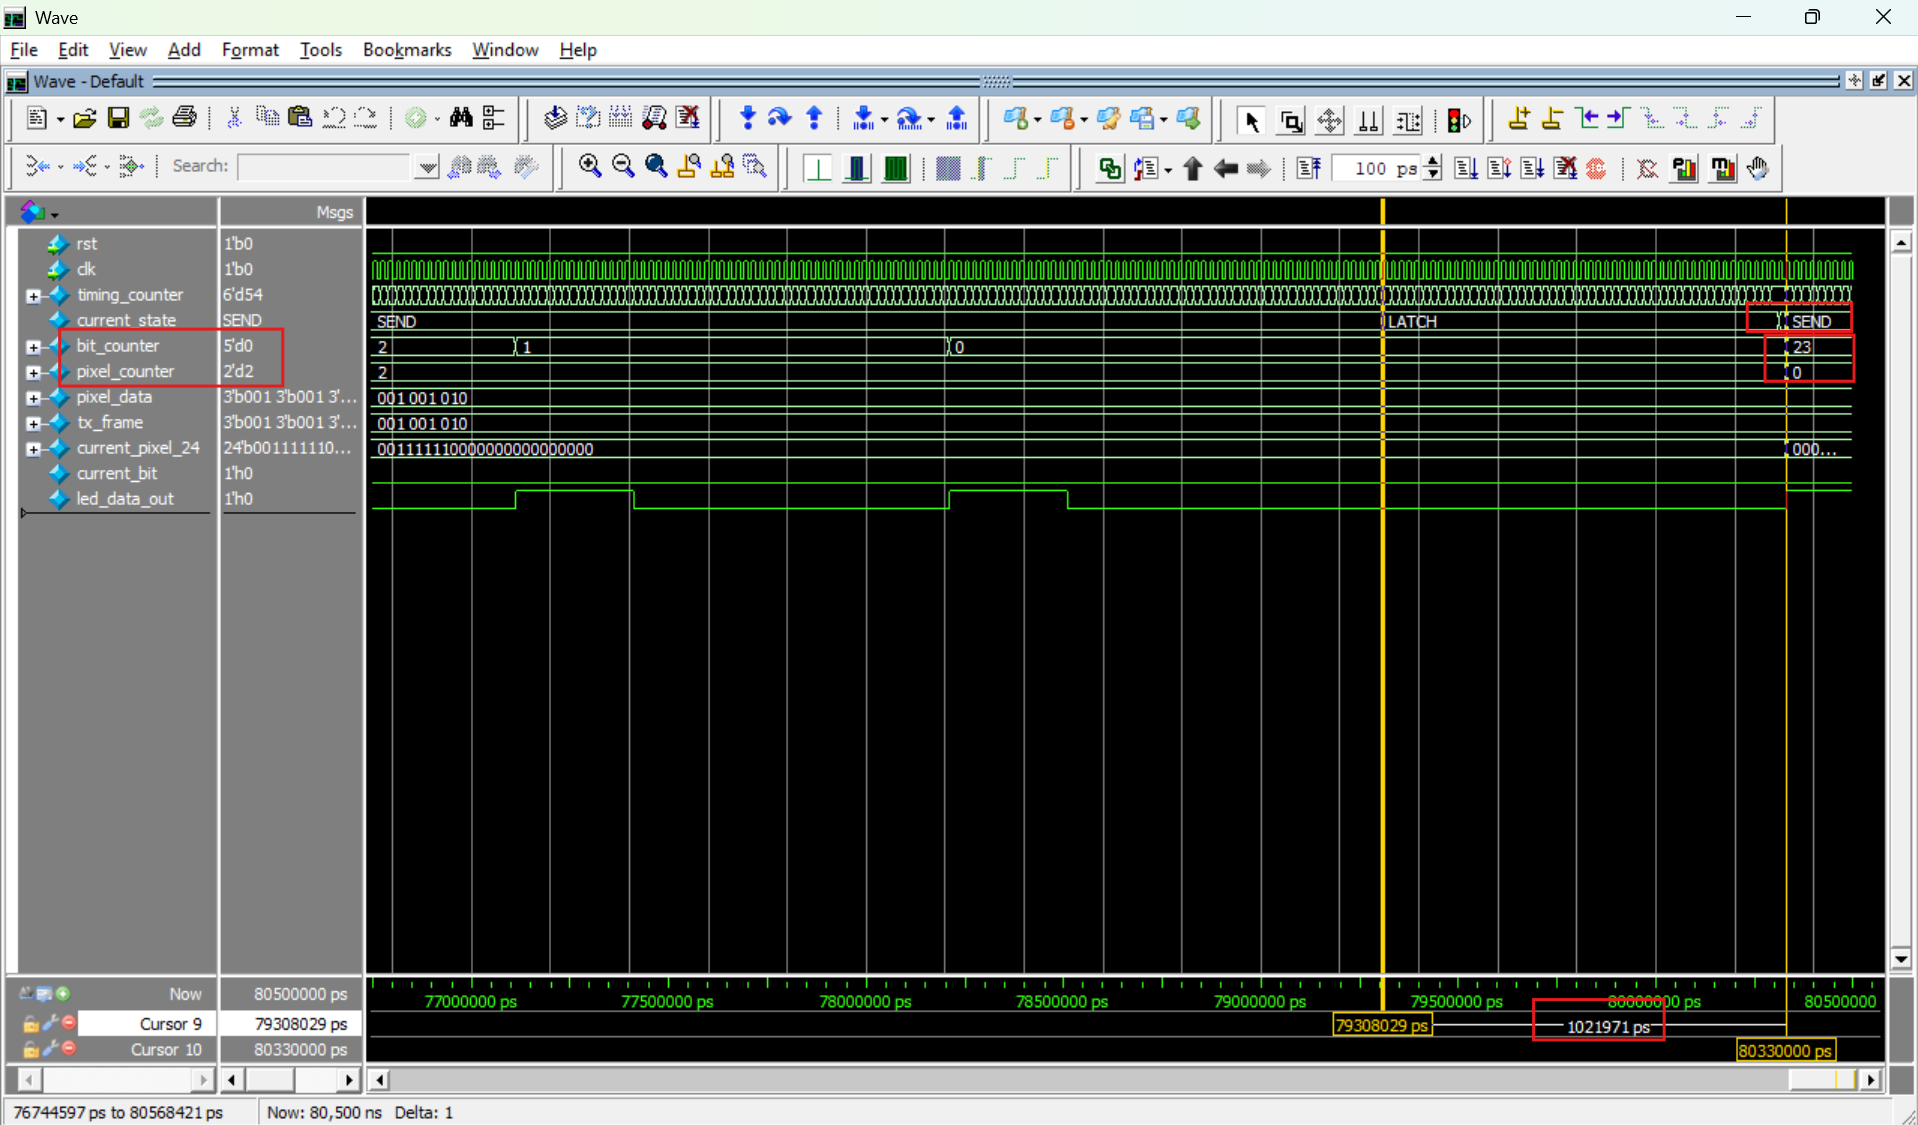
\includegraphics[width=\textwidth]{images/wf_tc05_latch_transition.png}
    \caption{Dạng sóng chuyển trạng thái SEND sang LATCH và giữ mức LOW trong thời gian RES}
    \label{fig:wf_tc05_latch}
\end{figure}

\subsubsection{Test Case 07: Cách ly Khung hình đang truyền (Snapshot Isolation)}
\begin{itemize}
    \item \textbf{Điều kiện kích thích:} Khi FSM đang thực thi trạng thái \texttt{SEND} (tại nhịp \texttt{timing\_counter = 2}), tín hiệu ngõ vào \texttt{pixel\_data} bị thay đổi đột ngột từ \texttt{\{001, 001, 010\}} sang \texttt{\{010, 011, 000\}}.
    \item \textbf{Phân tích dạng sóng:}
    \begin{itemize}
        \item Mặc dù ngõ vào \texttt{pixel\_data} bị cập nhật dữ liệu mới giữa chừng, mảng thanh ghi nội bộ \texttt{tx\_frame} vẫn giữ nguyên giá trị đã chốt trước đó là \texttt{\{001, 001, 010\}}.
        \item Bus dữ liệu 24-bit \texttt{current\_pixel\_24} tiếp tục duy trì giá trị \texttt{24'h003F00} (mã màu \texttt{RED}) tương ứng với phần tử \texttt{tx\_frame[0]} mà không bị ảnh hưởng bởi biến động đầu vào.
        \item Kết quả chứng minh kiến trúc chốt đệm \texttt{tx\_frame} đã thực hiện cô lập hoàn toàn khung truyền hình ảnh đang phát ra LED khỏi các cập nhật logic tức thời từ Game Engine, ngăn ngừa triệt để hiện tượng xé hình (frame tearing).
    \end{itemize}
\end{itemize}

\begin{figure}[H]
    \centering
    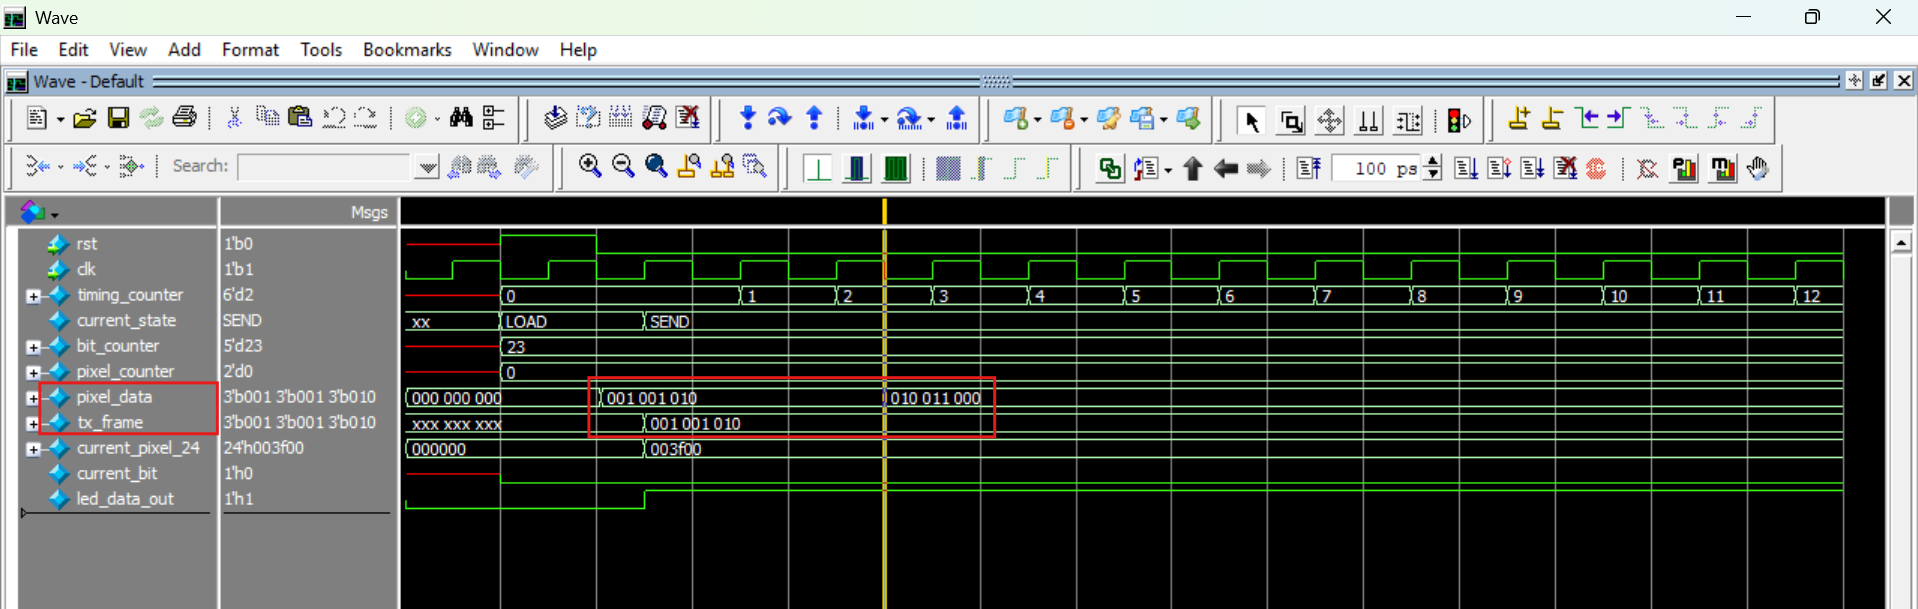
\includegraphics[width=\textwidth]{images/wf_tc07_snapshot_isolation.png}
    \caption{Dạng sóng kiểm tra tính cô lập dữ liệu: pixel\_data thay đổi giữa chừng nhưng tx\_frame và current\_pixel\_24 không bị ảnh hưởng}
    \label{fig:wf_tc07_snapshot}
\end{figure}

\newpage
\section{Button Conditioner}

Module \texttt{button\_conditioner} thực hiện đồng bộ tín hiệu từ các nút nhấn vật lý vào miền clock 50 MHz, phát hiện sự kiện nhấn và tạo tín hiệu \texttt{btn\_event} dạng xung một chu kỳ. Module được sử dụng làm giao tiếp giữa các nút nhấn của board DE2 và khối điều khiển \texttt{game\_engine}.

\textbf{Trạng thái:} Đã hoàn thiện RTL và kiểm tra chức năng cơ bản.


\section{Tick Generator}

Module \texttt{tick\_generator} sử dụng bộ đếm đồng bộ với clock 50 MHz để tạo các xung enable định kỳ cho hệ thống, gồm \texttt{bullet\_tick} với chu kỳ 50 ms và \texttt{snake\_tick} với chu kỳ 250 ms. Các tín hiệu này được sử dụng để điều khiển tốc độ cập nhật của bullet và snake trong \texttt{game\_engine}.

\textbf{Trạng thái:} Đã hoàn thiện RTL và kiểm tra chức năng cơ bản.
\newpage

\section{Kết quả Mô phỏng Module Game Engine}

\subsection{Mục tiêu Kiểm thử và Cấu hình Testbench}
Module \texttt{game\_engine} là khối xử lý trung tâm của hệ thống, đảm nhiệm quản lý máy trạng thái trò chơi (FSM), cập nhật tọa độ rắn (\textit{snake}), đạn (\textit{bullet}), giải quyết va chạm (\textit{collision}) và liên tục xuất mảng \texttt{pixel\_data} cho khối hiển thị.

Để tối ưu hóa thời gian mô phỏng trên ModelSim/QuestaSim (tránh phải chờ hàng triệu chu kỳ xung nhịp cho các chu kỳ thực tế 50 ms và 250 ms), môi trường kiểm thử (\texttt{game\_engine\_tb}) áp dụng cơ chế điều khiển xung tick mô phỏng rút gọn:
\begin{itemize}
    \item \textbf{Chu kỳ Master Clock:} $T_{\text{clk}} = 20\text{ ns}$ ($50\text{ MHz}$).
    \item \textbf{Độ phân giải thời gian mô phỏng:} \texttt{timescale 1ns/1ps}.
    \item \textbf{Cấu hình dải LED:} \texttt{LED\_COUNT} = 60 pixels, \texttt{DEFAULT\_LENGTH} = 5 segments.
    \item \textbf{Rút ngắn Timing bằng Simulation Ticks:} Thay vì chờ bộ đếm $2.5\times 10^6$ chu kỳ (50 ms cho \texttt{bullet\_tick}) và $12.5\times 10^6$ chu kỳ (250 ms cho \texttt{snake\_tick}), testbench trực tiếp tạo các xung tích cực mức cao kéo dài đúng 1 chu kỳ clock theo kịch bản để kích hoạt cập nhật động lực học trò chơi.
\end{itemize}

\subsection{Kế hoạch Kiểm thử Toàn diện (Verification Test Plan)}
Kế hoạch kiểm thử tập trung xác minh toàn bộ các quy tắc trò chơi, datapath tính toán look-ahead và máy trạng thái FSM thông qua 12 kịch bản:
\begin{enumerate}
    \item \textbf{TC01 -- Reset \& Initial State:} Kiểm tra tín hiệu reset đưa FSM về \texttt{IDLE}, rắn dài 5 đốt tại vị trí $55\rightarrow 59$ với đúng chuỗi màu, đạn ở trạng thái không tích cực (\texttt{bullet\_active} = 0).
    \item \textbf{TC02 -- IDLE $\rightarrow$ PLAYING:} Kiểm tra sự kiện nút nhấn đầu tiên kích hoạt chuyển trạng thái FSM sang \texttt{PLAYING} mà không bắn đạn ngay lập tức.
    \item \textbf{TC03 -- Snake Movement:} Kiểm tra tọa độ đầu rắn \texttt{head\_position} giảm 1 đơn vị và toàn bộ mảng \texttt{snake\_array} dịch chuyển chuẩn xác mỗi khi nhận xung \texttt{snake\_tick}.
    \item \textbf{TC04 -- Bullet Firing:} Kiểm tra sự kiện nhấn phím trong trạng thái \texttt{PLAYING} sinh đạn tại vị trí LED 0 với mã màu tương ứng (Red, Green, Blue, Yellow).
    \item \textbf{TC05 -- Bullet Movement:} Kiểm tra tọa độ đạn \texttt{bullet\_position} tăng dần từng bước theo mỗi xung \texttt{bullet\_tick}.
    \item \textbf{TC06 -- Same-color Collision:} Đạn chạm đầu rắn và trùng màu: đầu rắn bị tiêu biến, chiều dài rắn giảm 1 đơn vị, đạn bị vô hiệu hóa.
    \item \textbf{TC07 -- Different-color Collision:} Đạn chạm đầu rắn nhưng sai màu: chiều dài và màu sắc các đốt rắn giữ nguyên, đạn bị vô hiệu hóa.
    \item \textbf{TC08 -- WIN Condition:} Rắn bị tiêu diệt hoàn toàn (\texttt{snake\_length} = 0): FSM chuyển sang trạng thái \texttt{WIN}.
    \item \textbf{TC09 -- LOSE Condition:} Đầu rắn chạm mốc LED 0 (\texttt{head\_position} = 0): FSM chuyển sang trạng thái \texttt{LOSE}.
    \item \textbf{TC10 -- Simultaneous Tick / Look-Ahead:} Kiểm tra tính chính xác của khối Look-ahead khi \texttt{snake\_tick} và \texttt{bullet\_tick} kích hoạt đồng thời, chống hiện tượng xuyên đạn (\textit{Anti-Tunneling}).
    \item \textbf{TC11 -- Multiple Fire Prevention:} Khi đạn đang bay (\texttt{bullet\_active} = 1), mọi xung \texttt{btn\_event} bổ sung đều bị bỏ qua, không sinh thêm đạn.
    \item \textbf{TC12 -- Terminal State Behavior:} Tại trạng thái \texttt{WIN} hoặc \texttt{LOSE}, mọi chuyển động dừng hẳn và toàn dải \texttt{pixel\_data} render màu cố định (Solid Green cho WIN, Solid Red cho LOSE).
\end{enumerate}

\subsection{Bảng Tổng hợp Trạng thái Kiểm thử}
\begin{table}[H]
\centering
\caption{Bảng tổng hợp kết quả thực thi các Test Cases của Game Engine}
\label{tab:ge_summary}
\begin{tabular}{|c|l|p{7.5cm}|c|}
\hline
\textbf{STT} & \textbf{Kịch bản Kiểm thử} & \textbf{Tiêu chí Đánh giá} & \textbf{Kết quả} \\ \hline
\textbf{TC01} & Reset \& Initial State & FSM vào IDLE; Rắn dài 5 đốt (55--59); Đạn inactive & \textbf{PASS} \\ \hline
\textbf{TC02} & IDLE $\rightarrow$ PLAYING & Xung nút đầu tiên chuyển FSM sang PLAYING; Chưa sinh đạn & \textbf{PASS} \\ \hline
\textbf{TC03} & Snake Movement & \texttt{head\_position} giảm 1; Mảng dịch 1 vị trí khi có \texttt{snake\_tick} & \textbf{PASS} \\ \hline
\textbf{TC04} & Bullet Firing & Sinh đạn tại LED 0 đúng màu tương ứng với \texttt{btn\_event[3:0]} & \textbf{PASS} \\ \hline
\textbf{TC05} & Bullet Movement & \texttt{bullet\_position} tăng 1 vị trí mỗi khi có \texttt{bullet\_tick} & \textbf{PASS} \\ \hline
\textbf{TC06} & Same-color Collision & Trúng đạn cùng màu: \texttt{snake\_length} giảm 1; Đạn bị thu hồi & \textbf{PASS} \\ \hline
\textbf{TC07} & Different-color Collision & Sai màu: Thân rắn giữ nguyên; Đạn bị thu hồi & \textbf{PASS} \\ \hline
\textbf{TC08} & WIN Condition & \texttt{snake\_length} = 0 đưa FSM chuyển sang \texttt{WIN} & \textbf{PASS} \\ \hline
\textbf{TC09} & LOSE Condition & \texttt{head\_position} = 0 đưa FSM chuyển sang \texttt{LOSE} & \textbf{PASS} \\ \hline
\textbf{TC10} & Simultaneous Tick Look-Ahead & Xử lý va chạm chuẩn xác khi 2 tick đồng thời; Không bị vượt mặt & \textbf{PASS} \\ \hline
\textbf{TC11} & Multiple Fire Prevention & Nhấn nút khi \texttt{bullet\_active} = 1 không làm ghi đè đạn đang bay & \textbf{PASS} \\ \hline
\textbf{TC12} & Terminal State Behavior & Đóng băng cập nhật logic; Toàn dải xuất màu Solid GREEN / RED & \textbf{PASS} \\ \hline
\end{tabular}
\end{table}

\subsection{Bằng chứng Mô phỏng Thực tế (Waveform Evidence)}

\subsubsection{Test Case 01: Khởi tạo và Reset (Reset \& Initial State)}

\textbf{Mục tiêu:}
Kiểm tra phản hồi của hệ thống khi tín hiệu reset bất đồng bộ được kích hoạt, đảm bảo FSM chuyển về trạng thái \texttt{IDLE}, rắn được khởi tạo đúng độ dài và vị trí trên dải LED, đồng thời không có viên đạn nào ở trạng thái kích hoạt.

\textbf{Điều kiện kích thích:}
\begin{itemize}
    \item Tác động xung reset tích cực mức cao \texttt{rst\_sw = 1} trong 2 chu kỳ xung nhịp.
    \item Hạ \texttt{rst\_sw} về 0 tại cạnh âm của xung nhịp.
    \item Không tác động bất kỳ sự kiện nút nhấn nào (\texttt{btn\_event = 4'b0000}).
\end{itemize}

\textbf{Kết quả mong đợi:}
\begin{itemize}
    \item FSM chuyển về trạng thái \texttt{IDLE} (\texttt{current\_state = 2'b00}).
    \item Độ dài rắn \texttt{snake\_length} khởi tạo bằng 5.
    \item Vị trí đầu rắn \texttt{head\_position} khởi tạo tại LED 55.
    \item Các phần tử mảng thân rắn từ vị trí 55 đến 59 nạp đúng chuỗi màu mặc định: RED, GREEN, BLUE, YELLOW, RED.
    \item Trạng thái đạn không kích hoạt (\texttt{bullet\_active = 0}), \texttt{bullet\_position = 0}.
\end{itemize}

\textbf{Kết quả mô phỏng:}

Hình~\ref{fig:game-tc01} minh họa dạng sóng khi tác động tín hiệu reset lên module \texttt{game\_engine}. Ngay khi \texttt{rst\_sw} lên mức cao, FSM lập tức chuyển về trạng thái \texttt{IDLE}. Các thanh ghi cấu hình thân rắn được nạp chính xác với \texttt{head\_position = 55} và \texttt{snake\_length = 5}, các LED từ 55 đến 59 nhận các mã màu tương ứng. Đồng thời, cờ \texttt{bullet\_active} duy trì ở mức 0 và không có viên đạn nào xuất hiện trên dải LED.

\textbf{Kết luận:}
Test Case 01 đạt yêu cầu (PASS).

\begin{figure}[H]
    \centering
    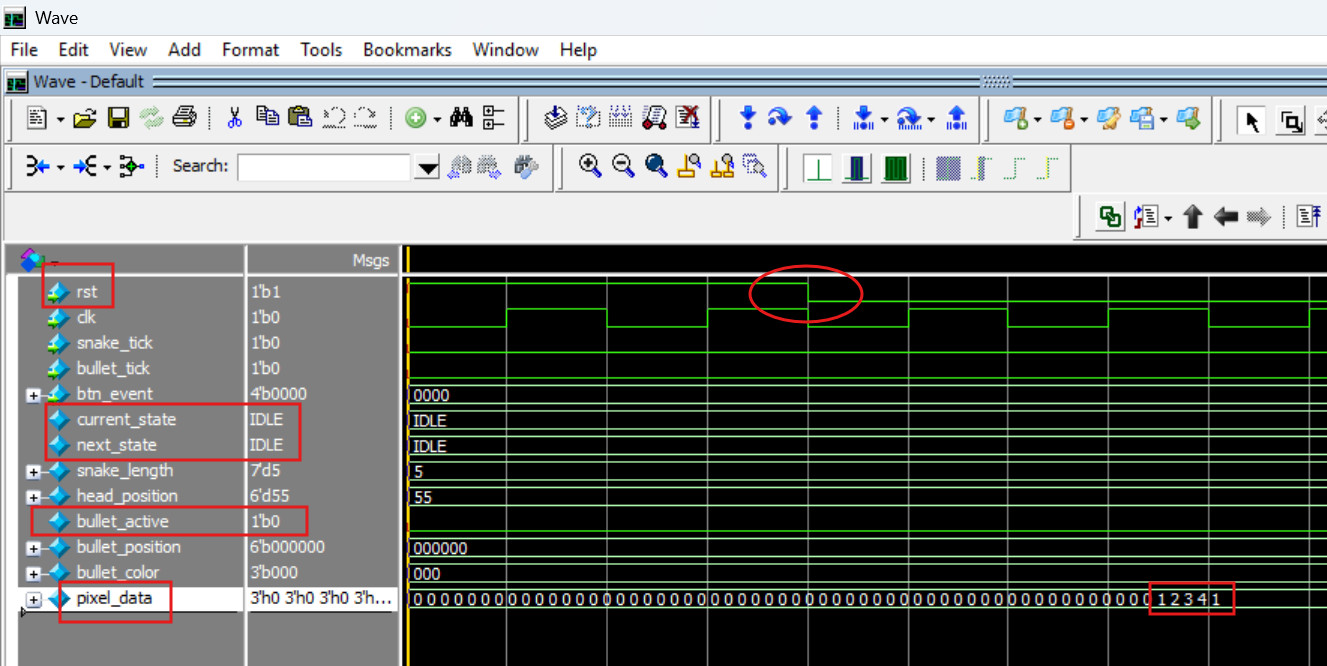
\includegraphics[width=0.95\textwidth]{images/game_engine_tc01_reset.png}
    \caption{Dạng sóng kiểm tra hành vi Reset và khởi tạo của Game Engine}
    \label{fig:game-tc01}
\end{figure}

\subsubsection{Test Case 02: Bắt đầu Trò chơi (IDLE $\rightarrow$ PLAYING)}

\textbf{Mục tiêu:}
Kiểm tra khả năng nhận diện sự kiện bắt đầu game của FSM khi có tín hiệu nhấn nút từ người chơi, đảm bảo hệ thống chuyển đúng từ trạng thái \texttt{IDLE} sang \texttt{PLAYING} mà không sinh đạn ngay trong chu kỳ đầu tiên.

\textbf{Điều kiện kích thích:}
\begin{itemize}
    \item Hệ thống đang duy trì ổn định ở trạng thái \texttt{IDLE} sau reset.
    \item Đưa một xung sự kiện nút nhấn \texttt{btn\_event[3] = 1} (phím màu YELLOW) kéo dài đúng 1 chu kỳ xung nhịp.
    \item Các tín hiệu \texttt{snake\_tick} và \texttt{bullet\_tick} chưa được kích hoạt.
\end{itemize}

\textbf{Kết quả mong đợi:}
\begin{itemize}
    \item FSM chuyển trạng thái từ \texttt{IDLE} sang \texttt{PLAYING} tại chu kỳ xung nhịp tiếp theo.
    \item Tín hiệu \texttt{bullet\_active} vẫn duy trì ở mức 0, chưa tạo đạn mới (nút nhấn ban đầu chỉ có tác dụng khởi động game).
    \item Tọa độ đầu rắn \texttt{head\_position} và chiều dài \texttt{snake\_length} không bị thay đổi.
\end{itemize}

\textbf{Kết quả mô phỏng:}

Hình~\ref{fig:game-tc02} mô tả đáp ứng của \texttt{game\_engine} khi nhận xung kích hoạt trò chơi. Ngay tại cạnh lên xung nhịp sau khi \texttt{btn\_event[3]} kích hoạt, biến trạng thái \texttt{current\_state} chuyển đổi chính xác sang \texttt{PLAYING}. Cờ \texttt{bullet\_active} tiếp tục giữ mức logic 0, chứng minh rằng sự kiện nút nhấn đầu tiên đã được FSM lọc đúng chức năng khởi động mà không gây hiện tượng bắn đạn ngoài ý muốn.

\textbf{Kết luận:}
Test Case 02 đạt yêu cầu (PASS).

\begin{figure}[H]
    \centering
    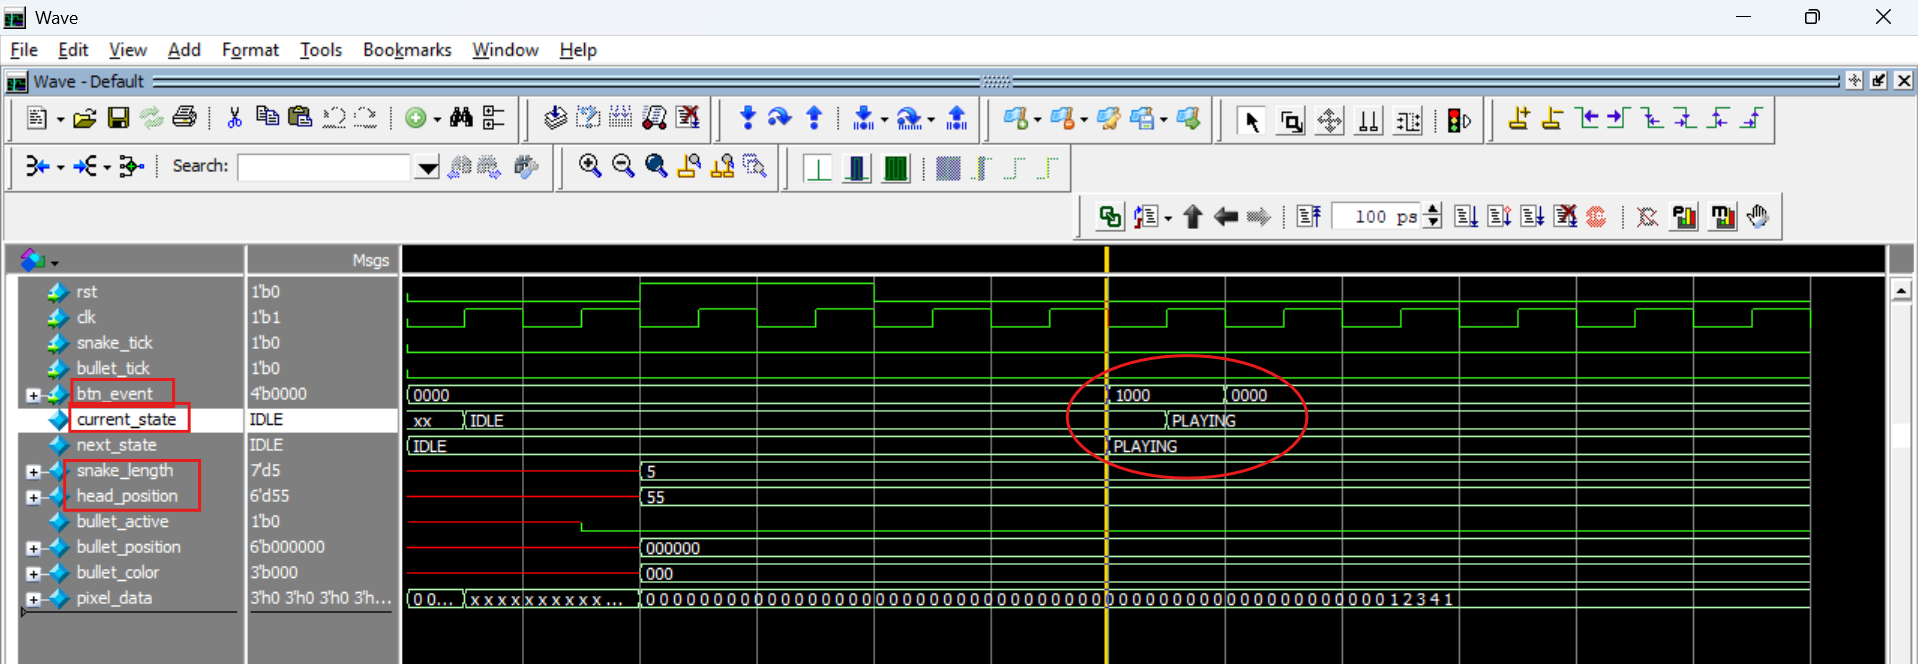
\includegraphics[width=0.95\textwidth]{images/game_engine_tc02_start.png}
    \caption{Dạng sóng kiểm tra chuyển trạng thái từ IDLE sang PLAYING}
    \label{fig:game-tc02}
\end{figure}

\subsubsection{Test Case 03: Động học Di chuyển của Rắn (Snake Movement)}

\textbf{Mục tiêu:}
Kiểm tra phản hồi của thân rắn khi có xung kích hoạt \texttt{snake\_tick}, đảm bảo vị trí đầu rắn \texttt{head\_position} giảm dần về phía LED 0 và toàn bộ mảng \texttt{snake\_array} được dịch chuyển chính xác theo nguyên lý thanh ghi dịch.

\textbf{Điều kiện kích thích:}
\begin{itemize}
    \item Hệ thống đang hoạt động ở trạng thái \texttt{PLAYING}.
    \item Đưa một xung \texttt{snake\_tick = 1} kéo dài đúng 1 chu kỳ xung nhịp.
    \item Tín hiệu \texttt{bullet\_tick = 0} và không có sự kiện nút nhấn (\texttt{btn\_event = 4'b0000}).
\end{itemize}

\textbf{Kết quả mong đợi:}
\begin{itemize}
    \item Tọa độ \texttt{head\_position} giảm đúng 1 đơn vị (từ 55 xuống 54) tại cạnh lên xung nhịp tiếp theo.
    \item Các phần tử trong mảng thân rắn thực hiện dịch chuyển sang trái (chỉ số thấp hơn) 1 vị trí.
    \item Chiều dài rắn \texttt{snake\_length} được bảo toàn nguyên vẹn (bằng 5).
    \item Thứ tự màu của các đốt thân rắn không bị sai lệch hay mất mát dữ liệu.
\end{itemize}

\textbf{Kết quả mô phỏng:}

Hình~\ref{fig:game-tc03} thể hiện dạng sóng di chuyển của rắn dưới tác động của xung định thời. Khi xuất hiện xung \texttt{snake\_tick}, bộ tính toán look-ahead cập nhật \texttt{next\_head = 54}. Tại cạnh lên tiếp theo của \texttt{clk}, thanh ghi \texttt{head\_position} cập nhật giá trị mới là 54, đồng thời mảng thanh ghi dịch thực hiện tịnh tiến toàn bộ các mã màu của thân rắn sang vị trí mới tương ứng. Độ dài \texttt{snake\_length} vẫn giữ nguyên giá trị 5, phản ánh chính xác hành vi di chuyển tự nhiên của rắn.

\textbf{Kết luận:}
Test Case 03 đạt yêu cầu (PASS).

\begin{figure}[H]
    \centering
    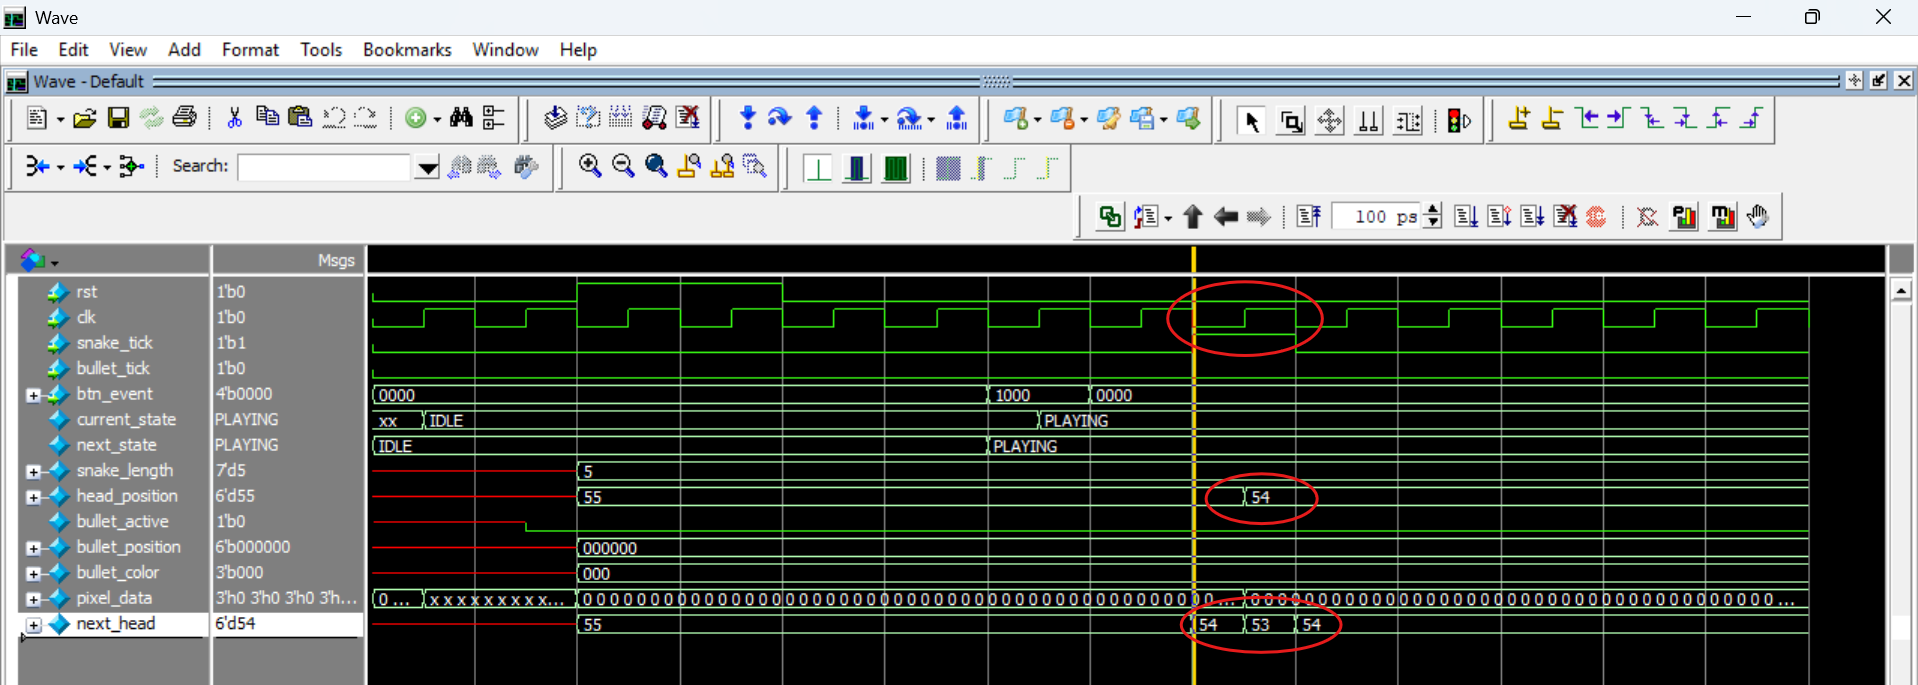
\includegraphics[width=0.95\textwidth]{images/game_engine_tc03_snake_move.png}
    \caption{Dạng sóng kiểm tra sự tịnh tiến của thân rắn theo xung snake\_tick}
    \label{fig:game-tc03}
\end{figure}

\subsubsection{Test Case 04: Tạo và Hiển thị Đạn (Bullet Firing \& Rendering)}

\textbf{Mục tiêu:}
Kiểm tra khả năng khởi tạo đạn khi người chơi nhấn nút trong trạng thái \texttt{PLAYING} và đảm bảo giá trị màu của đạn được ánh xạ lập tức lên mảng \texttt{pixel\_data} tại vị trí LED 0.

\textbf{Điều kiện kích thích:}
\begin{itemize}
    \item FSM đang ở trạng thái \texttt{PLAYING} và chưa có đạn hoạt động (\texttt{bullet\_active = 0}).
    \item Kích hoạt xung \texttt{btn\_event = 4'b0001} (phím màu RED) trong đúng 1 chu kỳ clock tại sườn âm.
    \item Sau 1 chu kỳ, hạ \texttt{btn\_event} về \texttt{4'b0000}.
\end{itemize}

\textbf{Kết quả mong đợi:}
\begin{itemize}
    \item Tín hiệu \texttt{bullet\_active} chuyển lên mức 1.
    \item Tọa độ khởi tạo \texttt{bullet\_position = 0} và màu đạn \texttt{bullet\_color = RED} (\texttt{3'b001}).
    \item Mảng hiển thị cập nhật chính xác: \texttt{pixel\_data[0] = RED} và \texttt{pixel\_data[1] = OFF}.
\end{itemize}

\textbf{Kết quả mô phỏng:}

Hình~\ref{fig:game-tc04} thể hiện dạng sóng quá trình sinh và render đạn màu RED. Sau khi nhận xung \texttt{btn\_event[0]}, module lập tức bật cờ \texttt{bullet\_active = 1}, gán \texttt{bullet\_position = 0} với mã màu RED. Mảng ngõ ra \texttt{pixel\_data[0]} nhận giá trị màu tương ứng ngay lập tức, trong khi LED 1 liền kề vẫn duy trì trạng thái tắt (OFF).

\textbf{Kết luận:}
Test Case 04 đạt yêu cầu (PASS).

\begin{figure}[H]
    \centering
    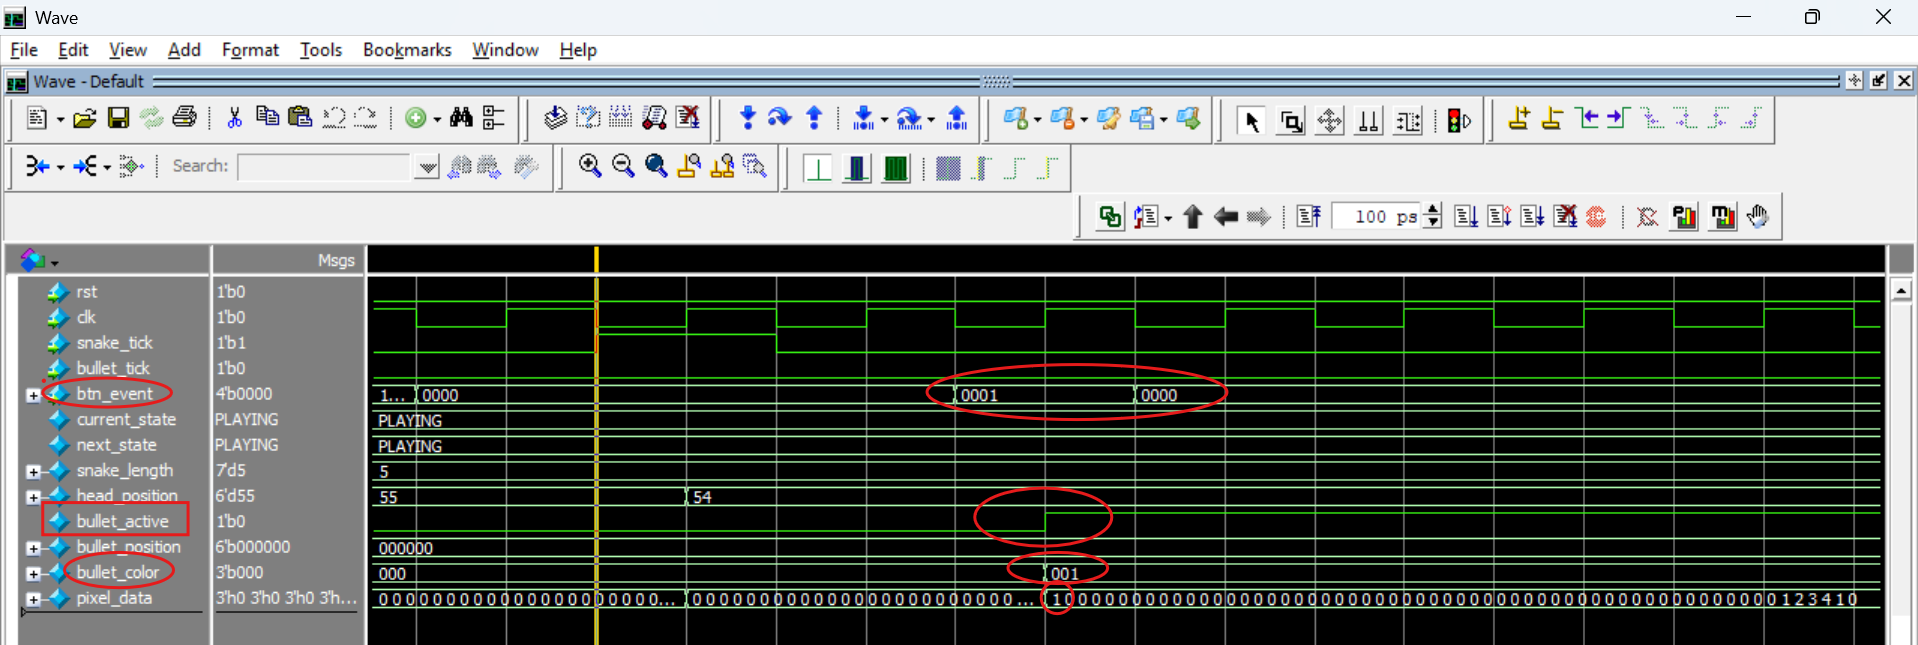
\includegraphics[width=0.95\textwidth]{images/game_engine_tc04_fire.png}
    \caption{Dạng sóng khởi tạo và hiển thị đạn màu RED tại LED 0}
    \label{fig:game-tc04}
\end{figure}

\subsubsection{Test Case 05: Động học Di chuyển của Đạn (Bullet Movement)}

\textbf{Mục tiêu:}
Kiểm tra phản hồi của đạn khi xuất hiện xung định thời \texttt{bullet\_tick}, đảm bảo tọa độ \texttt{bullet\_position} tịnh tiến chính xác dọc theo dải LED về phía chỉ số cao hơn và vị trí hiển thị trên mảng \texttt{pixel\_data} được cập nhật đồng thời.

\textbf{Điều kiện kích thích:}
\begin{itemize}
    \item Đạn màu RED đang ở trạng thái kích hoạt tại vị trí khởi tạo (\texttt{bullet\_active = 1}, \texttt{bullet\_position = 0}).
    \item Kích hoạt một xung \texttt{bullet\_tick = 1} kéo dài đúng 1 chu kỳ clock tại sườn âm của xung nhịp.
    \item Tín hiệu \texttt{snake\_tick = 0} và không có sự kiện nút nhấn mới (\texttt{btn\_event = 4'b0000}).
\end{itemize}

\textbf{Kết quả mong đợi:}
\begin{itemize}
    \item Tọa độ đạn \texttt{bullet\_position} tăng đúng 1 đơn vị (từ 0 lên 1) tại cạnh lên xung nhịp kế tiếp.
    \item Trạng thái kích hoạt và màu sắc đạn được duy trì ổn định (\texttt{bullet\_active = 1}, \texttt{bullet\_color = RED}).
    \item Mảng hiển thị LED dịch chuyển vị trí sáng tương ứng: \texttt{pixel\_data[0]} tắt (\texttt{OFF}) và \texttt{pixel\_data[1]} chuyển sang màu RED.
\end{itemize}

\textbf{Kết quả mô phỏng:}

Hình~\ref{fig:game-tc05} thể hiện dạng sóng di chuyển của đạn dưới tác động của \texttt{bullet\_tick}. Khi xung kích hoạt xuất hiện, bộ tính toán look-ahead gán giá trị dự đoán \texttt{next\_bullet = 1}. Tại cạnh lên tiếp theo của \texttt{clk}, thanh ghi \texttt{bullet\_position} cập nhật thành công lên 1, đồng thời vị trí hiển thị trên \texttt{pixel\_data} chuyển ngay từ LED 0 sang LED 1 mà không làm thay đổi trạng thái kích hoạt hay mã màu của đạn.

\textbf{Kết luận:}
Test Case 05 đạt yêu cầu (PASS).

\begin{figure}[H]
    \centering
    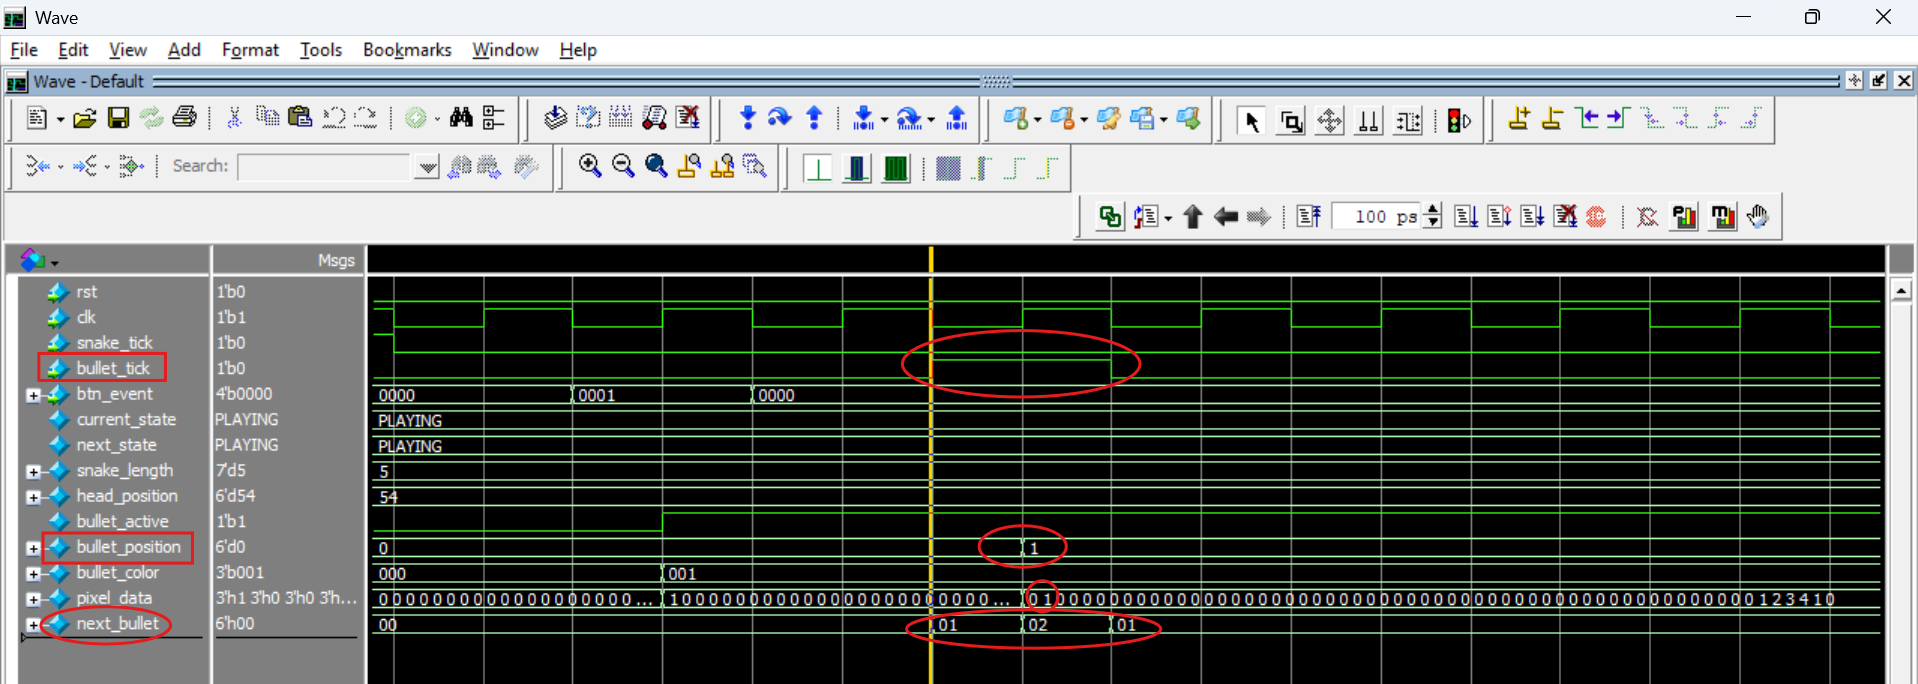
\includegraphics[width=0.95\textwidth]{images/game_engine_tc05_bullet_move.png}
    \caption{Dạng sóng kiểm tra sự tịnh tiến của đạn từ LED 0 sang LED 1 theo bullet\_tick}
    \label{fig:game-tc05}
\end{figure}

\subsubsection{Test Case 06: Va chạm Cùng Màu (Same-color Collision)}

\textbf{Mục tiêu:}
Kiểm tra phản hồi của hệ thống khi đạn va chạm với đầu rắn và có cùng màu sắc. Đốt đầu rắn tương ứng phải bị tiêu biến, chiều dài rắn giảm đi 1 đơn vị, đạn bị thu hồi về trạng thái không tích cực và FSM vẫn duy trì trạng thái \texttt{PLAYING} nếu rắn chưa bị diệt hết.

\textbf{Điều kiện kích thích:}
\begin{itemize}
    \item FSM đang ở trạng thái \texttt{PLAYING}.
    \item Đầu rắn đang có màu RED và tọa độ xác định (\texttt{head\_position}).
    \item Đạn màu RED đang hoạt động (\texttt{bullet\_active = 1}, \texttt{bullet\_color = RED}).
    \item Đạn được dịch chuyển đến vị trí chạm trán với đầu rắn thông qua xung tick.
\end{itemize}

\textbf{Kết quả mong đợi:}
\begin{itemize}
    \item Điều kiện va chạm được kích hoạt thành công.
    \item Chiều dài thân rắn \texttt{snake\_length} giảm đi 1 đơn vị (từ 5 về 4).
    \item Vị trí đầu rắn cũ bị xóa bỏ khỏi mảng hiển thị.
    \item Cờ \texttt{bullet\_active} chuyển từ 1 về 0 (đạn biến mất sau va chạm).
    \item Trạng thái FSM tiếp tục duy trì ở \texttt{PLAYING}.
\end{itemize}

\textbf{Kết quả mô phỏng:}

Hình~\ref{fig:game-tc06} thể hiện dạng sóng quá trình xử lý va chạm trúng khi đạn và đầu rắn trùng màu. Khi đạn tiếp cận vị trí của đầu rắn, bộ giải mã va chạm xác nhận sự kiện trùng màu. Tại chu kỳ cập nhật tiếp theo, thanh ghi \texttt{snake\_length} giảm tức thì từ 5 xuống 4, đồng thời đốt đầu cũ bị gỡ bỏ khỏi mảng logic. Đạn được vô hiệu hóa an toàn bằng cách hạ cờ \texttt{bullet\_active} về 0 mà không gây xung nhiễu lên các vị trí LED khác.

\textbf{Kết luận:}
Test Case 06 đạt yêu cầu (PASS).

\begin{figure}[H]
    \centering
    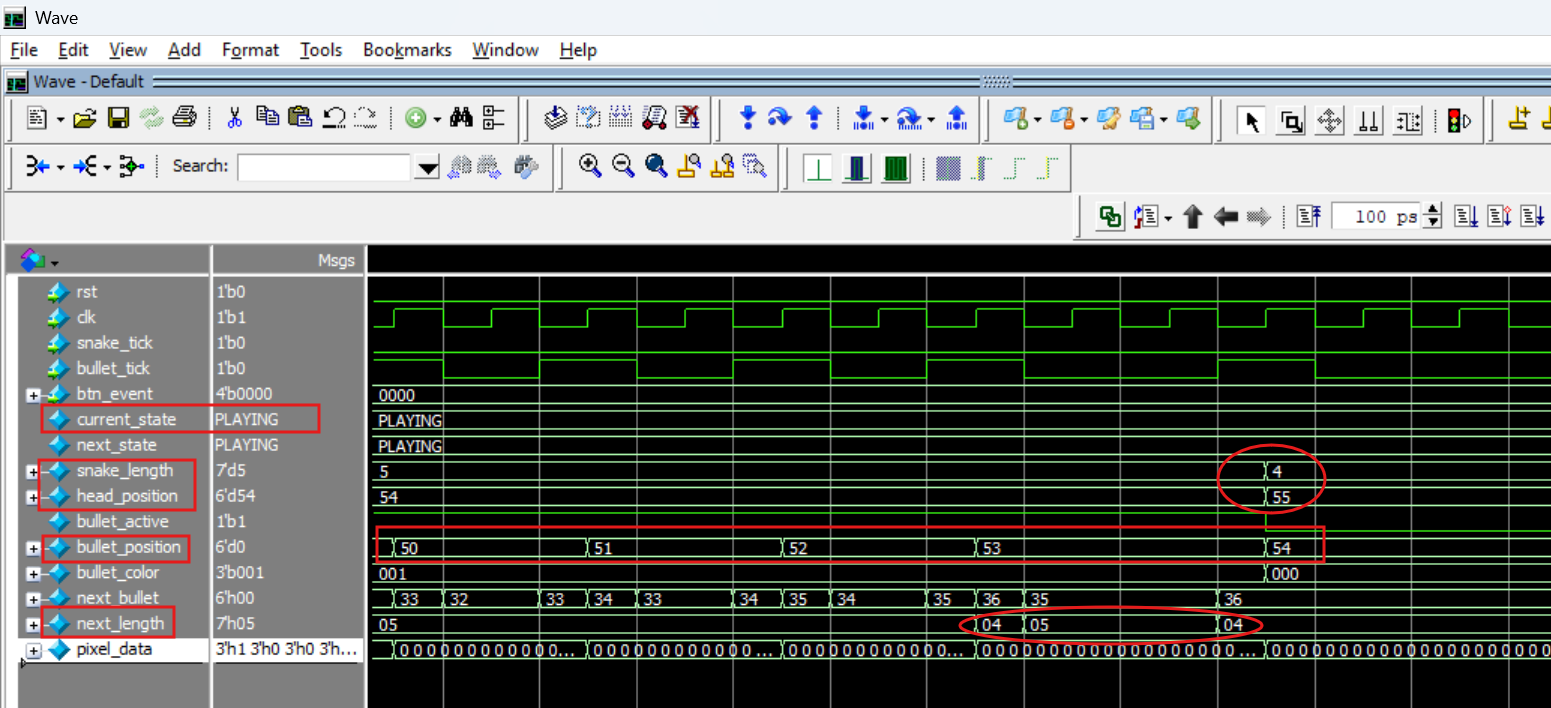
\includegraphics[width=0.95\textwidth]{images/game_engine_tc06_collision.png}
    \caption{Dạng sóng kiểm tra va chạm cùng màu giữa đạn và đầu rắn}
    \label{fig:game-tc06}
\end{figure}

\subsubsection{Test Case 07: Va chạm Khác Màu (Different-color Collision)}

\textbf{Mục tiêu:}
Kiểm tra khả năng phân biệt màu sắc khi xảy ra va chạm: nếu màu đạn không trùng khớp với màu của đầu rắn, đạn phải bị thu hồi ngay lập tức, trong khi thân rắn, chiều dài và màu sắc các đốt của rắn được giữ nguyên vẹn.

\textbf{Điều kiện kích thích:}
\begin{itemize}
    \item FSM đang ở trạng thái \texttt{PLAYING}.
    \item Đầu rắn hiện tại mang mã màu RED (\texttt{3'b001}).
    \item Kích hoạt một viên đạn mang màu YELLOW (\texttt{bullet\_color = 3'b100}) đến vị trí chạm trán với đầu rắn.
    \item Bơm các xung \texttt{bullet\_tick} tuần tự để đẩy đạn tới sát đầu rắn, sau đó kích hoạt 1 xung \texttt{bullet\_tick} cuối cùng để tạo va chạm trúng màu.
\end{itemize}

\textbf{Kết quả mong đợi:}
\begin{itemize}
    \item Mạch phát hiện va chạm xác lập sự kiện nhưng nhận diện kết quả sai màu (mismatch).
    \item Chiều dài thân rắn \texttt{snake\_length} giữ nguyên không đổi.
    \item Mảng thân rắn \texttt{snake\_array} và vị trí đầu rắn giữ nguyên các giá trị ban đầu.
    \item Tín hiệu \texttt{bullet\_active} chuyển về mức 0 (đạn bị vô hiệu hóa).
    \item Trạng thái FSM tiếp tục duy trì ở \texttt{PLAYING}.
\end{itemize}

\textbf{Kết quả mô phỏng:}

Hình~\ref{fig:game-tc07} ghi nhận dạng sóng phản hồi khi đạn va chạm sai màu với đầu rắn. Khi đạn YELLOW tiếp xúc với đầu rắn RED, bộ giải mã logic nhận diện sự bất đồng bộ về màu sắc. Tại cạnh lên xung nhịp cập nhật trạng thái, cờ \texttt{bullet\_active} được kéo về 0 để giải phóng làn đạn, đồng thời thanh ghi \texttt{snake\_length} không hề bị suy giảm và vị trí hiển thị của rắn trên \texttt{pixel\_data} được bảo toàn nguyên vẹn.

\textbf{Kết luận:}
Test Case 07 đạt yêu cầu (PASS).

\begin{figure}[H]
    \centering
    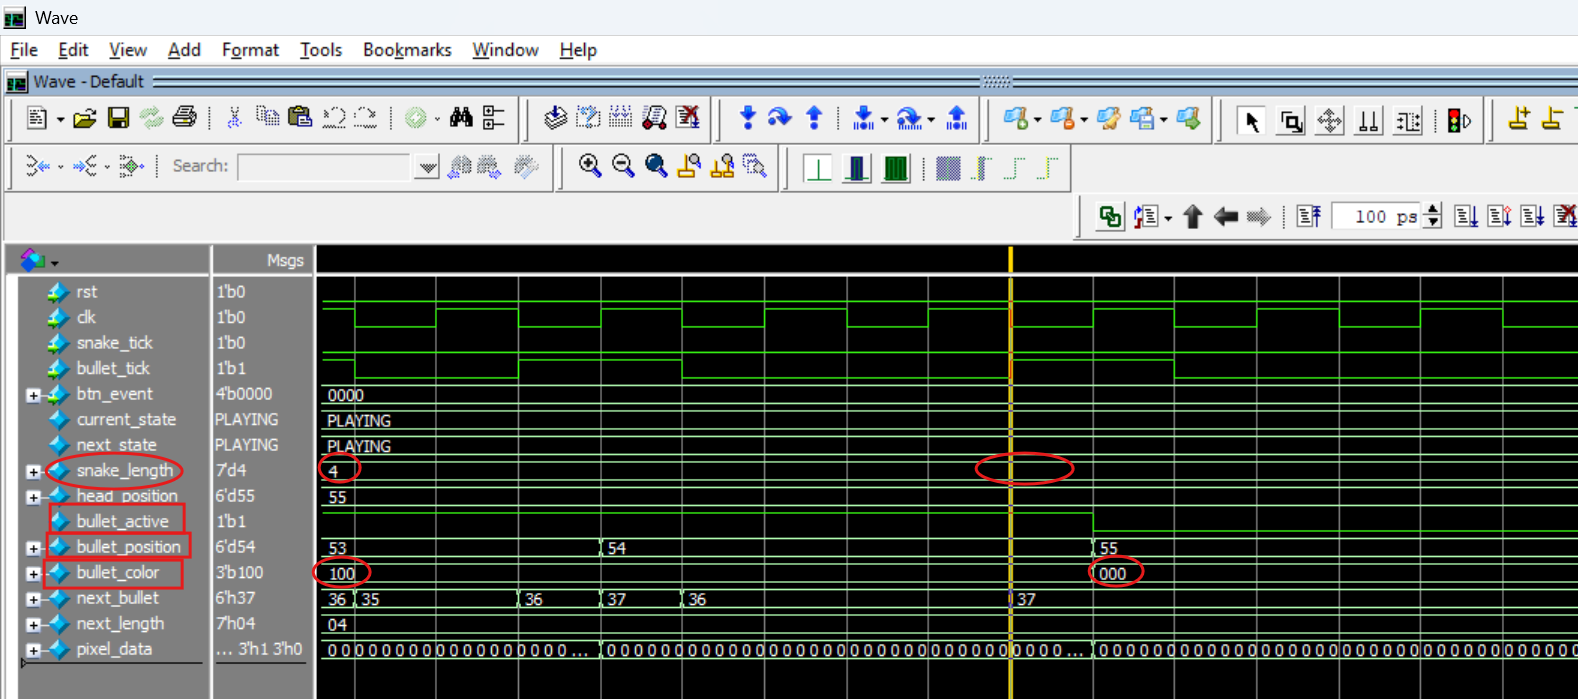
\includegraphics[width=0.95\textwidth]{images/game_engine_tc07_collision_diff.png}
    \caption{Dạng sóng kiểm tra va chạm khác màu giữa đạn và đầu rắn}
    \label{fig:game-tc07}
\end{figure}

\subsubsection{Test Case 08: Kích hoạt Điều kiện Thắng (WIN Condition)}

\textbf{Mục tiêu:}
Kiểm tra khả năng nhận diện điều kiện chiến thắng của FSM thông qua quy trình bắn hạ liên tục toàn bộ các đốt thân rắn cho đến khi chiều dài rắn giảm về 0 (\texttt{snake\_length = 0}).

\textbf{Điều kiện kích thích:}
\begin{itemize}
    \item Hệ thống đang chạy ở trạng thái \texttt{PLAYING}.
    \item Sử dụng vòng lặp tự động trong testbench: đọc mã màu tại đầu rắn \texttt{snake\_array[head\_position]} và phát xung \texttt{btn\_event} tạo đạn có màu tương ứng.
    \item Bơm các xung \texttt{bullet\_tick} tuần tự để đẩy đạn tới sát đầu rắn, sau đó kích hoạt 1 xung \texttt{bullet\_tick} cuối cùng để tạo va chạm trúng màu.
    \item Lặp lại quy trình triệt tiêu trên cho đến khi toàn bộ các đốt rắn bị loại bỏ.
\end{itemize}

\textbf{Kết quả mong đợi:}
\begin{itemize}
    \item Độ dài thân rắn giảm tuần tự sau mỗi lần bắn trúng và đạt \texttt{snake\_length = 0}.
    \item FSM lập tức chuyển từ trạng thái \texttt{PLAYING} sang trạng thái \texttt{WIN} (\texttt{current\_state == WIN}).
    \item Không còn viên đạn nào ở trạng thái kích hoạt sau khi rắn bị tiêu diệt hết.
\end{itemize}

\textbf{Kết quả mô phỏng:}

Hình~\ref{fig:game-tc08-loop} và Hình~\ref{fig:game-tc08-win} minh họa toàn bộ tiến trình tự động bắn hạ thân rắn và chuyển đổi trạng thái FSM. Dưới sự điều phối của testbench, từng đốt rắn bị triệt tiêu tương ứng sau mỗi pha va chạm cùng màu. Sau khi \texttt{snake\_length} giảm về 0, FSM chuyển sang trạng thái WIN ở chu kỳ cập nhật kế tiếp.

\textbf{Kết luận:}
Test Case 08 đạt yêu cầu (PASS).

\begin{figure}[H]
    \centering
    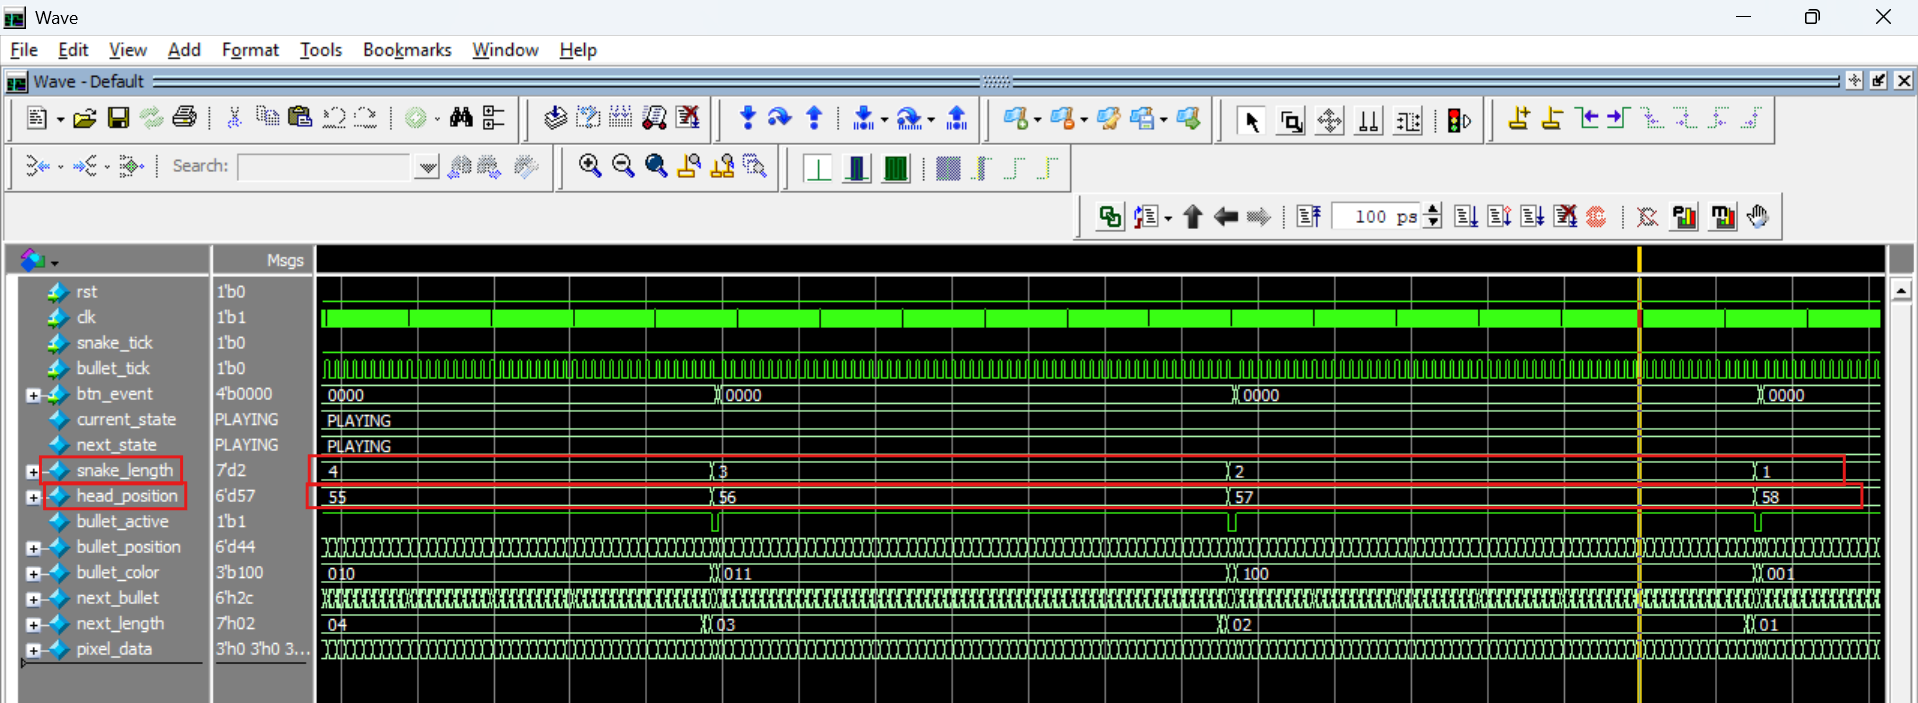
\includegraphics[width=0.95\textwidth]{images/game_engine_tc08_loop.png}
    \caption{Dạng sóng tiến trình tự động bắn trúng và triệt tiêu từng đốt rắn}
    \label{fig:game-tc08-loop}
\end{figure}

\begin{figure}[H]
    \centering
    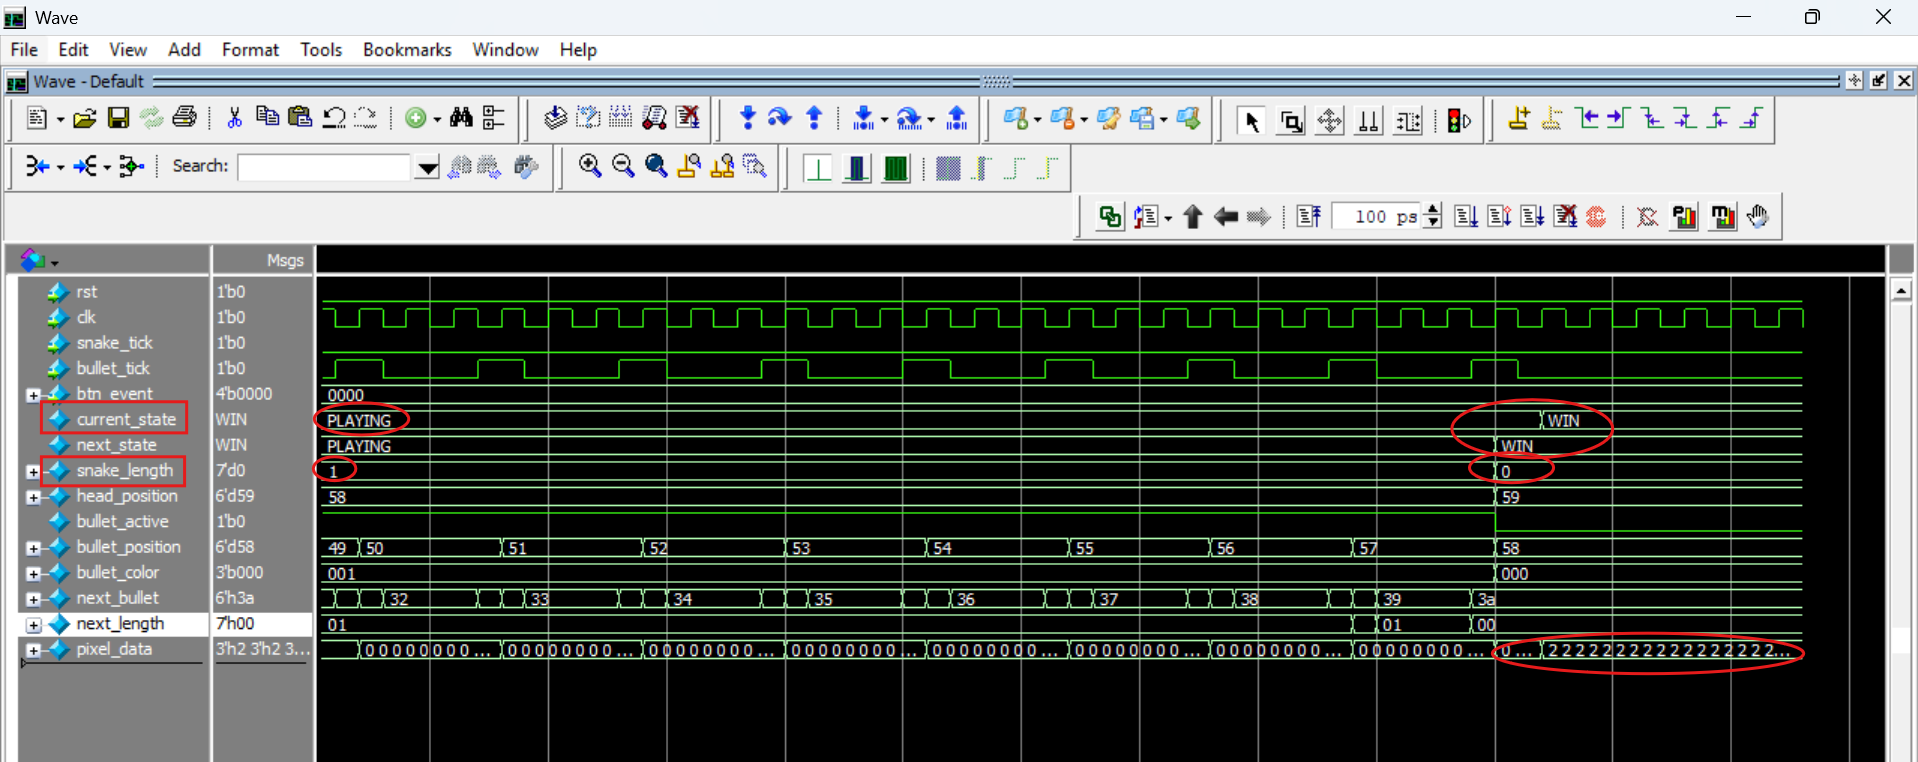
\includegraphics[width=0.95\textwidth]{images/game_engine_tc08_win.png}
    \caption{Dạng sóng kiểm tra snake\_length về 0 và FSM chuyển sang trạng thái WIN}
    \label{fig:game-tc08-win}
\end{figure}

\subsubsection{Test Case 09: Kích hoạt Điều kiện Thua (LOSE Condition)}

\textbf{Mục tiêu:}
Kiểm tra khả năng phát hiện điều kiện thua cuộc của FSM khi đầu rắn tịnh tiến chạm mốc biên giới hạn LED 0 (\texttt{head\_position = 0}), đảm bảo hệ thống chuyển chính xác từ trạng thái \texttt{PLAYING} sang \texttt{LOSE} và khóa các hoạt động di chuyển tiếp theo.

\textbf{Điều kiện kích thích:}
\begin{itemize}
    \item Reset lại hệ thống sau trạng thái \texttt{WIN} của TC08 bằng xung \texttt{rst = 1} trong 2 chu kỳ xung nhịp.
    \item Đưa xung \texttt{btn\_event = 4'b1000} (YELLOW) trong 1 chu kỳ clock để chuyển FSM từ \texttt{IDLE} sang \texttt{PLAYING}.
    \item Bơm liên tục các xung \texttt{snake\_tick} thông qua vòng lặp \texttt{while} để đẩy đầu rắn tịnh tiến từ vị trí ban đầu (55) về vị trí LED 1.
    \item Kích hoạt một xung \texttt{snake\_tick} quyết định cuối cùng để đưa đầu rắn vào vị trí LED 0.
\end{itemize}

\textbf{Kết quả mong đợi:}
\begin{itemize}
    \item Tọa độ đầu rắn chạm biên LED 0: \texttt{head\_position == 0}.
    \item FSM chuyển trạng thái tức thì từ \texttt{PLAYING} sang \texttt{LOSE} (\texttt{current\_state == LOSE}).
    \item Hệ thống khóa điều khiển, không cho phép đầu rắn tiếp tục giảm xuống dưới 0.
\end{itemize}

\textbf{Kết quả mô phỏng:}

Hình~\ref{fig:game-tc09-move} và Hình~\ref{fig:game-tc09-lose} minh họa tiến trình tịnh tiến của thân rắn về phía LED 0 và thời điểm kích hoạt trạng thái \texttt{LOSE}. Sau khi hoàn tất reset và chuyển sang \texttt{PLAYING}, các xung \texttt{snake\_tick} đẩy dần \texttt{head\_position} từ 55 về 1. Ngay tại cạnh lên xung nhịp nhận xung tick cuối cùng, \texttt{head\_position} đạt giá trị 0, đồng thời biến trạng thái \texttt{current\_state} chuyển đổi sang \texttt{LOSE} ở clock kế tiếp, đáp ứng đúng tiêu chí đánh giá kiểm thử.

\textbf{Kết luận:}
Test Case 09 đạt yêu cầu (PASS).

\begin{figure}[H]
    \centering
    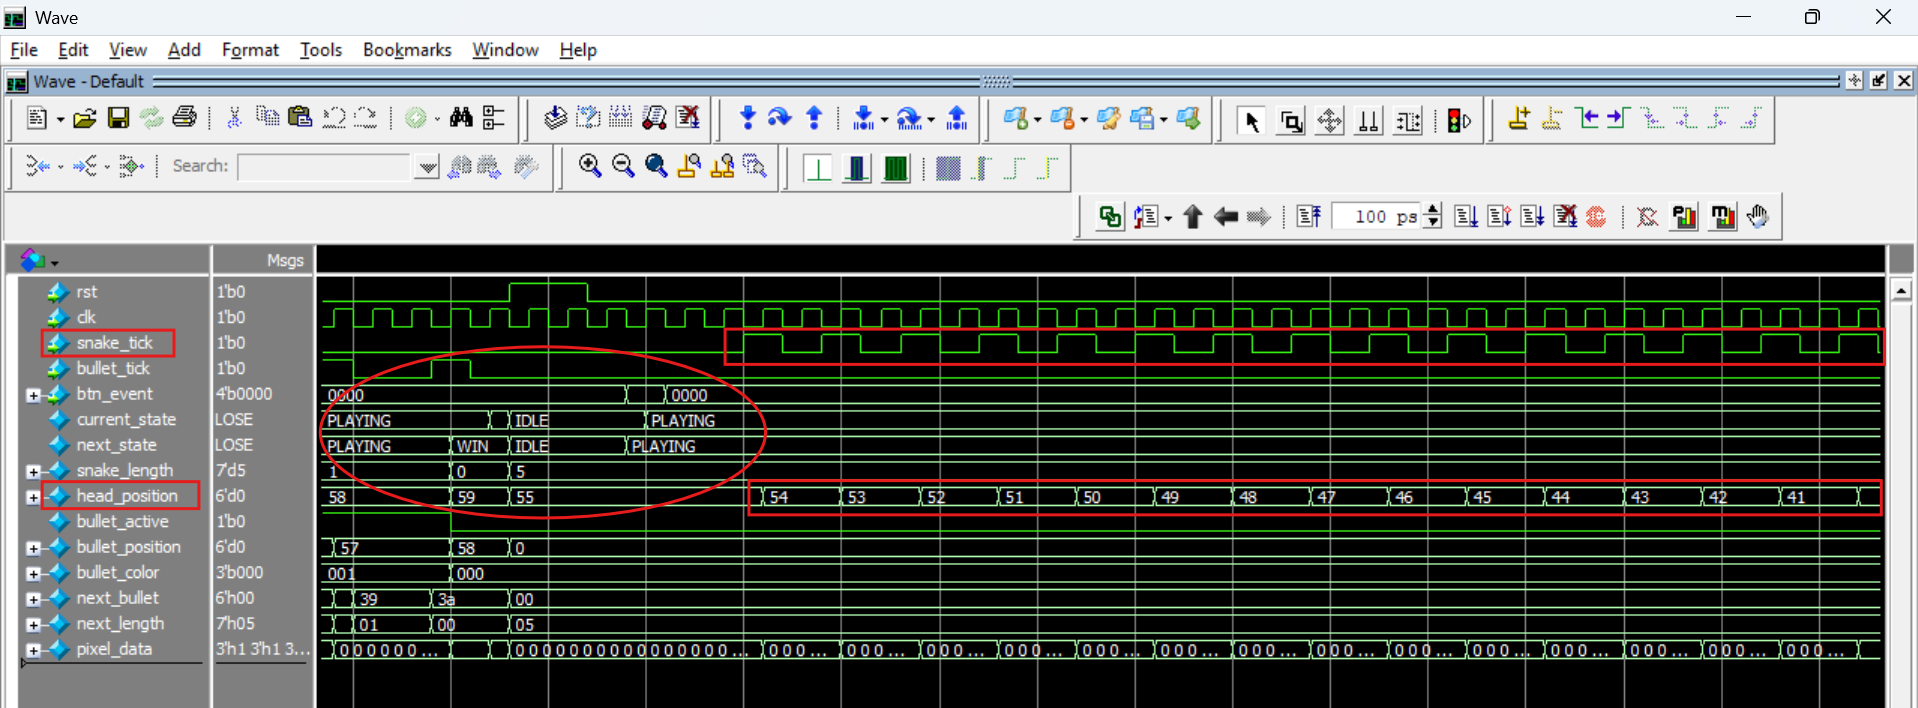
\includegraphics[width=0.95\textwidth]{images/game_engine_tc09_move.png}
    \caption{Dạng sóng quá trình tịnh tiến liên tục của rắn về phía LED 0}
    \label{fig:game-tc09-move}
\end{figure}

\begin{figure}[H]
    \centering
    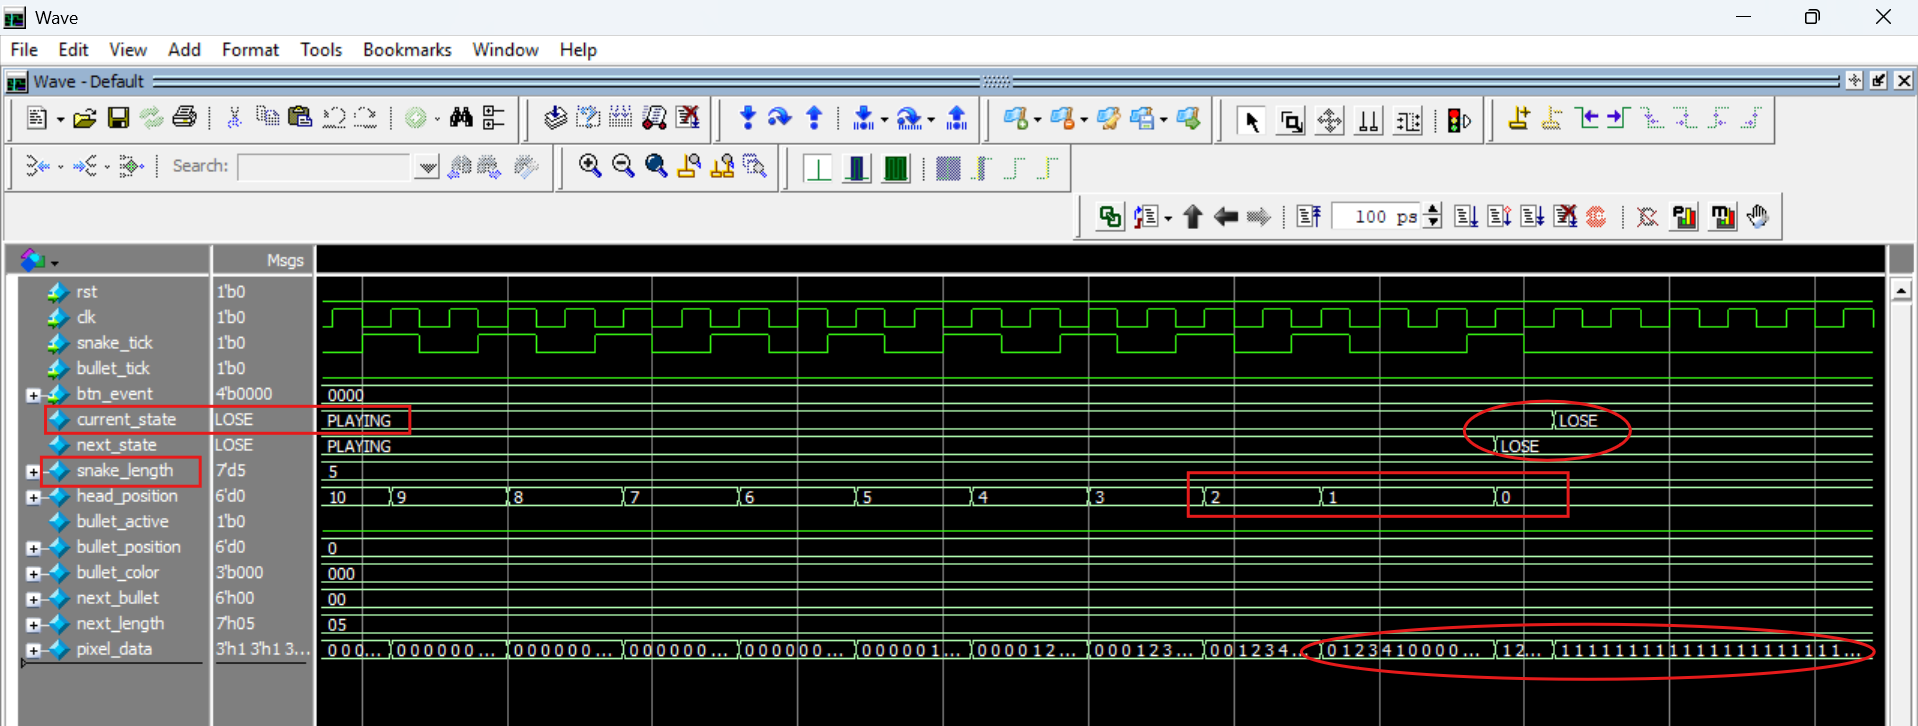
\includegraphics[width=0.95\textwidth]{images/game_engine_tc09_lose.png}
    \caption{Dạng sóng head\_position chạm LED 0 và FSM chuyển sang LOSE}
    \label{fig:game-tc09-lose}
\end{figure}

\subsubsection{Test Case 10: Khởi động lại từ Trạng thái Thua (Restart from LOSE)}

\textbf{Mục tiêu:}
Kiểm tra khả năng khôi phục toàn diện của hệ thống khi nhận tín hiệu reset từ trạng thái kết thúc \texttt{LOSE}, đảm bảo FSM quay về \texttt{IDLE}, các thông số vị trí và độ dài thân rắn được nạp lại cấu hình mặc định ban đầu, đồng thời xóa bỏ hoàn toàn trạng thái đạn.

\textbf{Điều kiện kích thích:}
\begin{itemize}
    \item Hệ thống đang bị đóng băng tại trạng thái kết thúc \texttt{LOSE} từ TC09.
    \item Tác động xung reset tích cực mức cao \texttt{rst = 1} trong 2 chu kỳ xung nhịp tại sườn âm của clock.
    \item Hạ \texttt{rst} về 0 và quan sát sự tái lập trạng thái của module.
\end{itemize}

\textbf{Kết quả mong đợi:}
\begin{itemize}
    \item FSM thoát khỏi \texttt{LOSE} và quay về trạng thái an toàn \texttt{IDLE} (\texttt{current\_state == IDLE}).
    \item Chiều dài thân rắn khôi phục về giá trị mặc định: \texttt{snake\_length == LENGTH\_TEST} (5 segments).
    \item Tọa độ đầu rắn được đặt lại tại vị trí xuất phát: \texttt{head\_position == LED\_TEST - LENGTH\_TEST} (LED 55).
    \item Trạng thái đạn được xóa bỏ hoàn toàn (\texttt{bullet\_active == 0}).
\end{itemize}

\textbf{Kết quả mô phỏng:}

Hình~\ref{fig:game-tc10} thể hiện dạng sóng quá trình giải phóng trạng thái khóa và tái thiết lập hệ thống từ trạng thái \texttt{LOSE}. Ngay khi \texttt{rst} được kích hoạt, máy trạng thái FSM lập tức chuyển từ \texttt{LOSE} về \texttt{IDLE}. Các thanh ghi điều khiển được nạp lại đầy đủ các thông số khởi tạo chuẩn (\texttt{snake\_length} = 5, \texttt{head\_position} = 55), đồng thời cờ \texttt{bullet\_active} được xóa về 0, đưa hệ thống sẵn sàng cho lượt chơi mới.

\textbf{Kết luận:}
Test Case 10 đạt yêu cầu (PASS).

\begin{figure}[H]
    \centering
    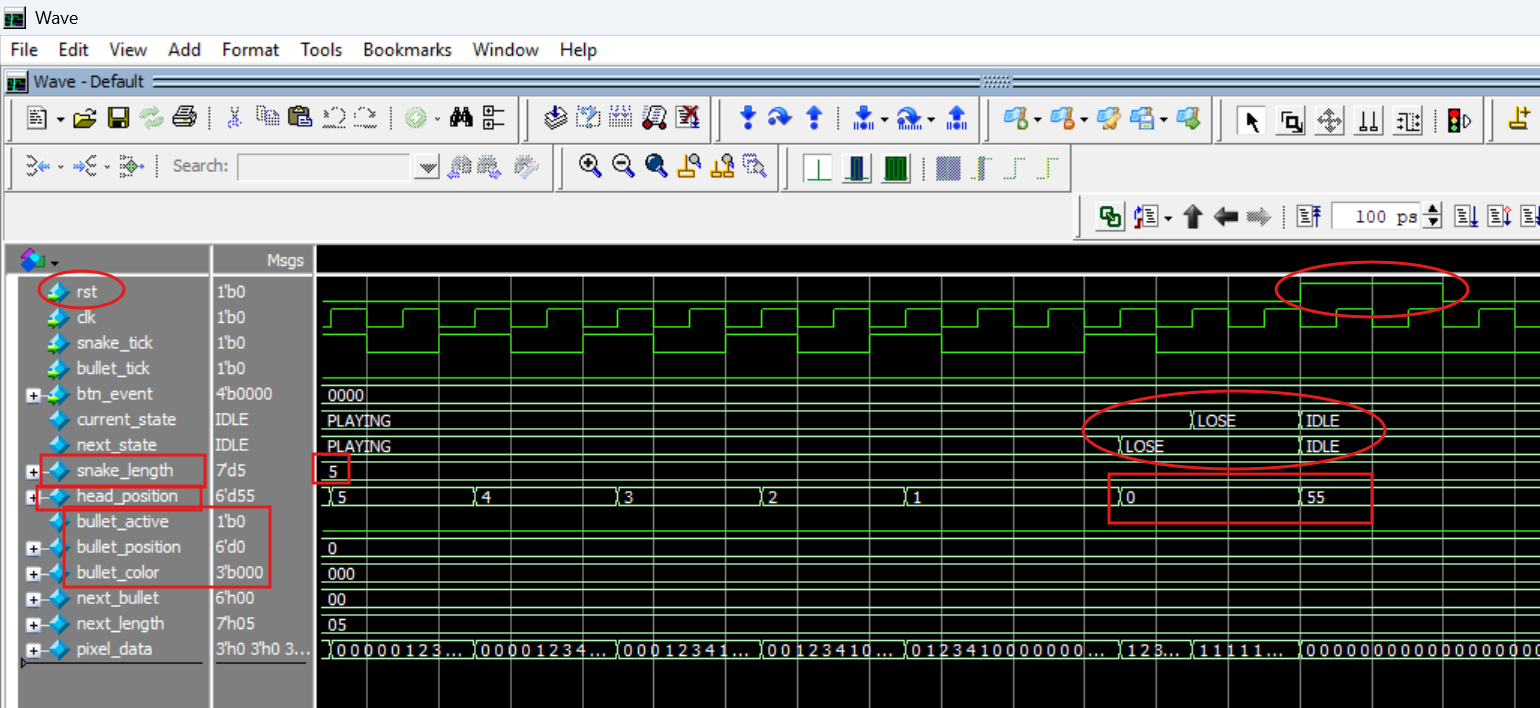
\includegraphics[width=0.95\textwidth]{images/game_engine_tc10_restart_lose.png}
    \caption{Dạng sóng khôi phục hệ thống về IDLE từ trạng thái LOSE sau khi Reset}
    \label{fig:game-tc10}
\end{figure}

\subsubsection{Test Case 11: Xung Kích hoạt Đồng thời (Simultaneous Ticks)}

\textbf{Mục tiêu:}
Kiểm tra tính toàn vẹn của logic cập nhật trạng thái khi cả hai xung \texttt{bullet\_tick} và \texttt{snake\_tick} cùng tích cực trong một chu kỳ xung nhịp. Đánh giá hai giai đoạn: chuyển động tịnh tiến đồng thời và va chạm trực diện trong cùng một chu kỳ tick kép (kiểm tra cơ chế Anti-Tunneling).

\textbf{Điều kiện kích thích:}
\begin{itemize}
    \item Chuyển FSM sang \texttt{PLAYING} và tạo một viên đạn màu RED tại LED 0 (\texttt{bullet\_active = 1}).
    \item \textbf{Giai đoạn 1 (Chuyển động đồng thời):} Kích hoạt đồng thời \texttt{bullet\_tick = 1} và \texttt{snake\_tick = 1} trong 1 chu kỳ clock.
    \item Bơm các xung \texttt{bullet\_tick} đơn để đẩy đạn đến sát đầu rắn (\texttt{bullet\_position < head\_position - 1}).
    \item \textbf{Giai đoạn 2 (Va chạm tick kép):} Kích hoạt đồng thời \texttt{bullet\_tick = 1} và \texttt{snake\_tick = 1} ngay tại thời điểm đạn và đầu rắn đối đầu trực tiếp.
\end{itemize}

\textbf{Kết quả mong đợi:}
\begin{itemize}
    \item \textbf{Tại Giai đoạn 1:} Đạn tịnh tiến lên LED 1; rắn tịnh tiến về dải LED 54--58, LED 59 tắt (\texttt{OFF}); mảng \texttt{pixel\_data} render đồng thời cả đạn và thân rắn chính xác.
    \item \textbf{Tại Giai đoạn 2:} Va chạm được phát hiện tức thì; \texttt{bullet\_active} về 0, mã màu đạn chuyển về \texttt{OFF}; độ dài \texttt{snake\_length} giảm đi 1; vị trí đầu \texttt{head\_position} dời sang LED 55 (đốt đầu đỏ tại LED 54 bị xóa); mảng LED cập nhật chính xác với LED 53, 54 tắt và các đốt còn lại hiển thị GREEN (55), BLUE (56), YELLOW (57), RED (58).
\end{itemize}

\textbf{Kết quả mô phỏng:}

Hình~\ref{fig:game-tc11-move} và Hình~\ref{fig:game-tc11-collision} minh họa chi tiết hai pha kiểm thử của Test Case 11. Ở pha đầu tiên, đạn và thân rắn đều dịch chuyển đồng thời 1 vị trí mà không gây xung đột tín hiệu. Ở pha va chạm, dù cả đạn và đầu rắn cùng tịnh tiến đối đầu trong cùng một chu kỳ clock, mạch Look-ahead đã giải quyết va chạm chính xác: đốt đầu đỏ tại LED 54 bị triệt tiêu, đạn biến mất và đầu rắn mới dời về vị trí 55 mà không xảy ra hiện tượng đạn bị xuyên qua thân rắn.

\textbf{Kết luận:}
Test Case 11 đạt yêu cầu (PASS).

\begin{figure}[H]
    \centering
    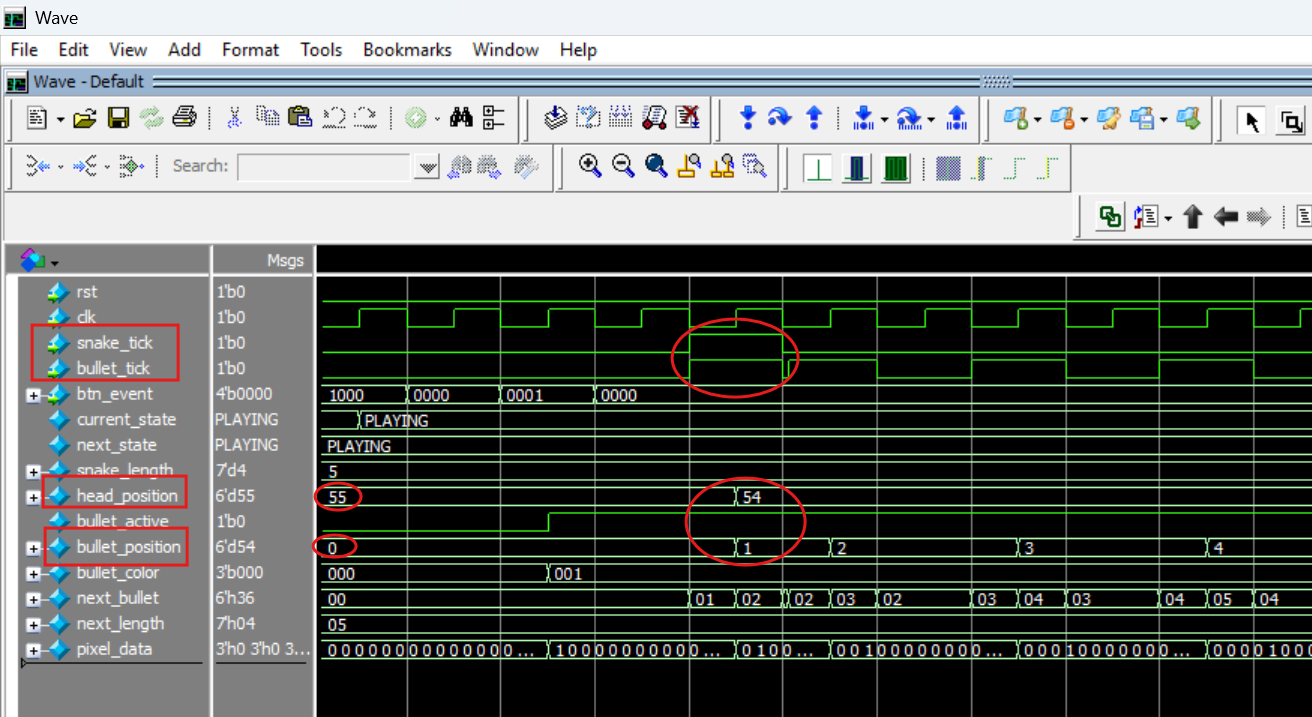
\includegraphics[width=0.95\textwidth]{images/game_engine_tc11_move.png}
    \caption{Dạng sóng dịch chuyển đồng thời của đạn và rắn khi kích hoạt tick kép}
    \label{fig:game-tc11-move}
\end{figure}

\begin{figure}[H]
    \centering
    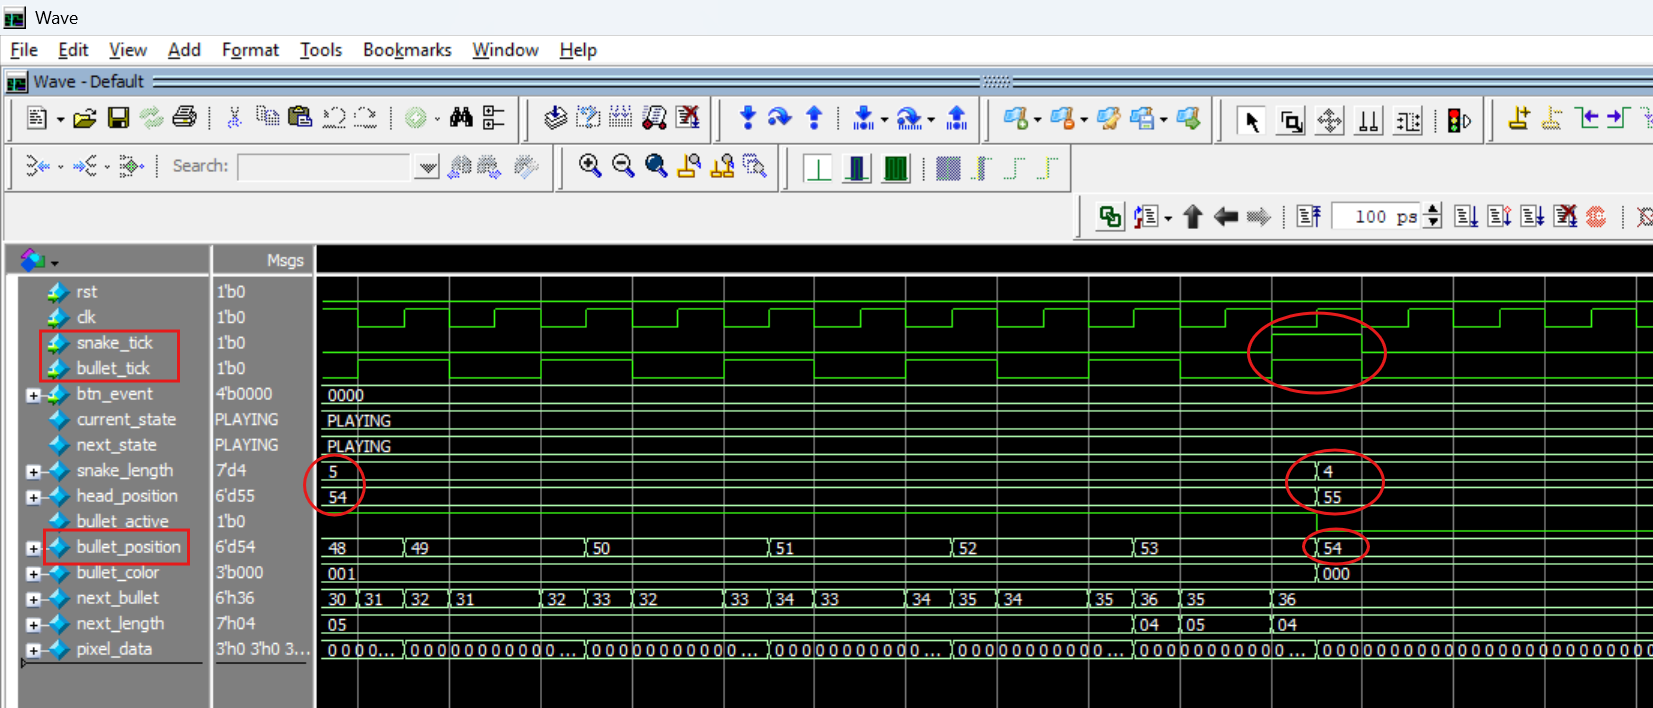
\includegraphics[width=0.95\textwidth]{images/game_engine_tc11_collision.png}
    \caption{Dạng sóng xử lý va chạm trúng cùng màu trong cùng chu kỳ kích hoạt tick kép}
    \label{fig:game-tc11-collision}
\end{figure}

\subsubsection{Test Case 12: Chống Bắn Đạn Dồn Dập (Rapid Fire Prevention Stress Test)}

\textbf{Mục tiêu:}
Kiểm tra khả năng bảo vệ hệ thống trước các thao tác nhấn phím bất thường khi đang có một viên đạn bay trên dải LED (\texttt{bullet\_active = 1}): nhấn ngẫu nhiên liên tục, nhấn tổ hợp nhiều phím cùng lúc, và giữ đè phím trong nhiều chu kỳ xung nhịp. Đảm bảo viên đạn đang bay không bị biến dạng về màu sắc hay vị trí, và không có viên đạn mới nào bị sinh đè lên vị trí LED 0.

\textbf{Điều kiện kích thích:}
\begin{itemize}
    \item Bắn một viên đạn màu GREEN (\texttt{bullet\_color = 3'b010}) và cấp 3 xung \texttt{bullet\_tick} để đẩy đạn tới vị trí LED 3 (\texttt{bullet\_position = 3}).
    \item \textbf{Pha 1 (Spam ngẫu nhiên):} Kích hoạt xung phím ngẫu nhiên \texttt{4'b0001 << \$urandom\_range(0,3)} liên tiếp trong 3 chu kỳ clock.
    \item \textbf{Pha 2 (Tổ hợp phím):} Kích hoạt đồng thời toàn bộ các phím (\texttt{btn\_event = 4'b1111}) trong 1 chu kỳ clock.
    \item \textbf{Pha 3 (Giữ đè phím):} Giữ đè phím RED (\texttt{btn\_event = 4'b0001}) liên tục trong suốt 5 chu kỳ clock.
    \item \textbf{Pha 4 (Kiểm tra LED 0):} Quan sát giá trị xuất ra của \texttt{pixel\_data[0]} trong suốt các pha tác động trên.
\end{itemize}

\textbf{Kết quả mong đợi:}
\begin{itemize}
    \item Viên đạn GREEN đang bay hoàn toàn miễn nhiễm với mọi kích thích nút bấm: \texttt{bullet\_color} giữ nguyên màu GREEN. Trong điều kiện không có \texttt{bullet\_tick}, các \texttt{btn\_event} bổ sung không làm thay đổi \texttt{bullet\_position}, \texttt{bullet\_color} hoặc \texttt{bullet\_active}.
    \item Không có bất kỳ viên đạn mới nào được nạp vào mảng hiển thị: \texttt{pixel\_data[0] == OFF} (LED 0 luôn giữ trạng thái tắt).
\end{itemize}

\textbf{Kết quả mô phỏng:}

Hình~\ref{fig:game-tc12-spam} và Hình~\ref{fig:game-tc12-hold} ghi nhận phản hồi của module trong các pha kiểm thử ứng suất nút nhấn. Khi một viên đạn GREEN đã được bắn ra và di chuyển đến vị trí LED 3, mọi hành vi spam ngẫu nhiên, bấm tổ hợp nhiều phím cùng lúc, hay giữ đè phím RED đều bị logic điều khiển chặn lại an toàn. Vị trí và mã màu của viên đạn đang bay duy trì ổn định tuyệt đối. Đồng thời, \texttt{pixel\_data[0]} giữ mức \texttt{OFF} xuyên suốt quá trình thử nghiệm, chứng minh cơ chế chỉ cho phép duy nhất một viên đạn hoạt động trên dải LED hoạt động chính xác và tin cậy.

\textbf{Kết luận:}
Test Case 12 đạt yêu cầu (PASS).

\begin{figure}[H]
    \centering
    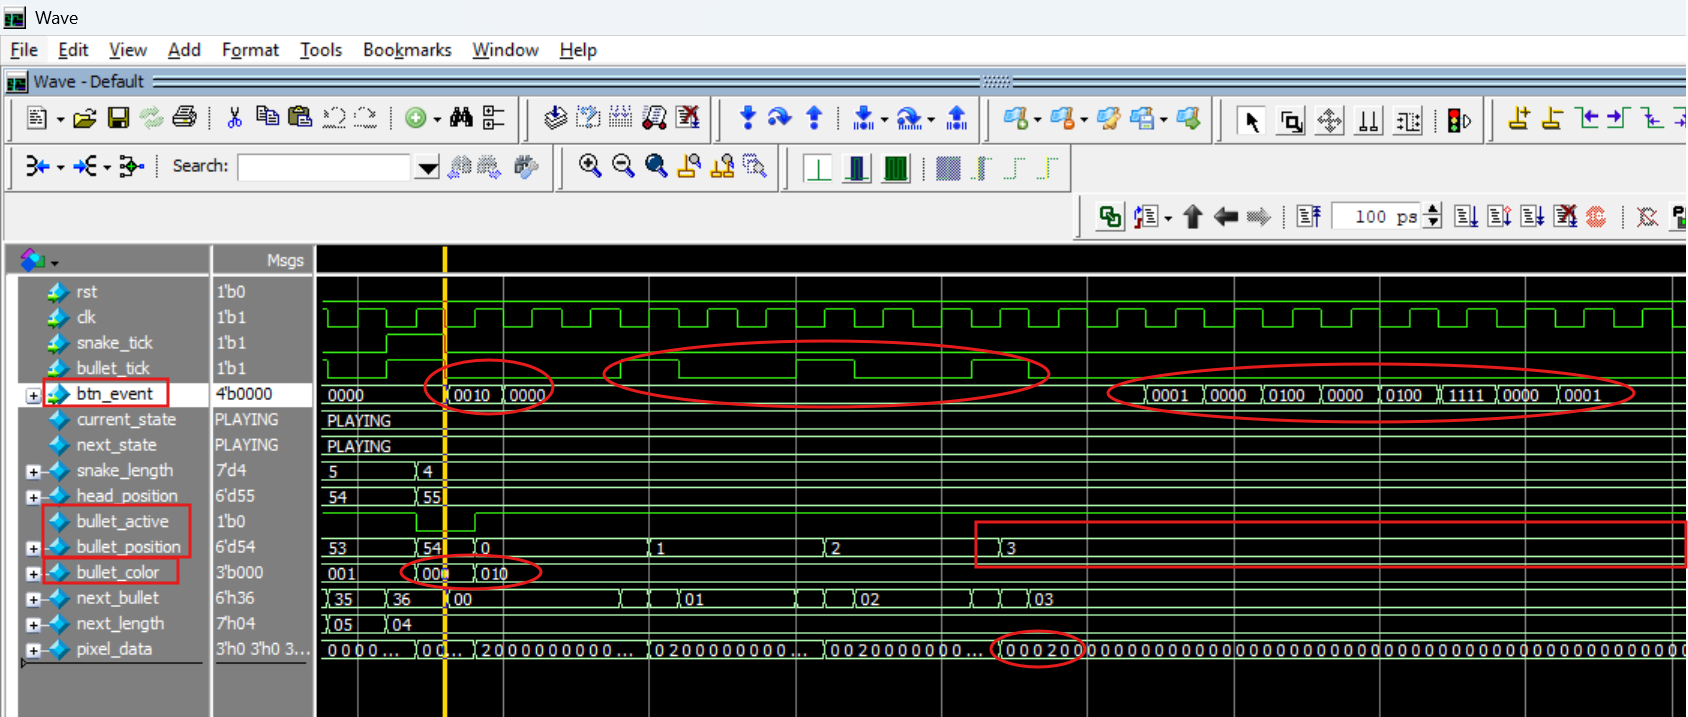
\includegraphics[width=0.95\textwidth]{images/game_engine_tc12_spam_multi.png}
    \caption{Dạng sóng kiểm tra tính cô lập của đạn khi spam nút ngẫu nhiên và bấm tổ hợp phím}
    \label{fig:game-tc12-spam}
\end{figure}

\begin{figure}[H]
    \centering
    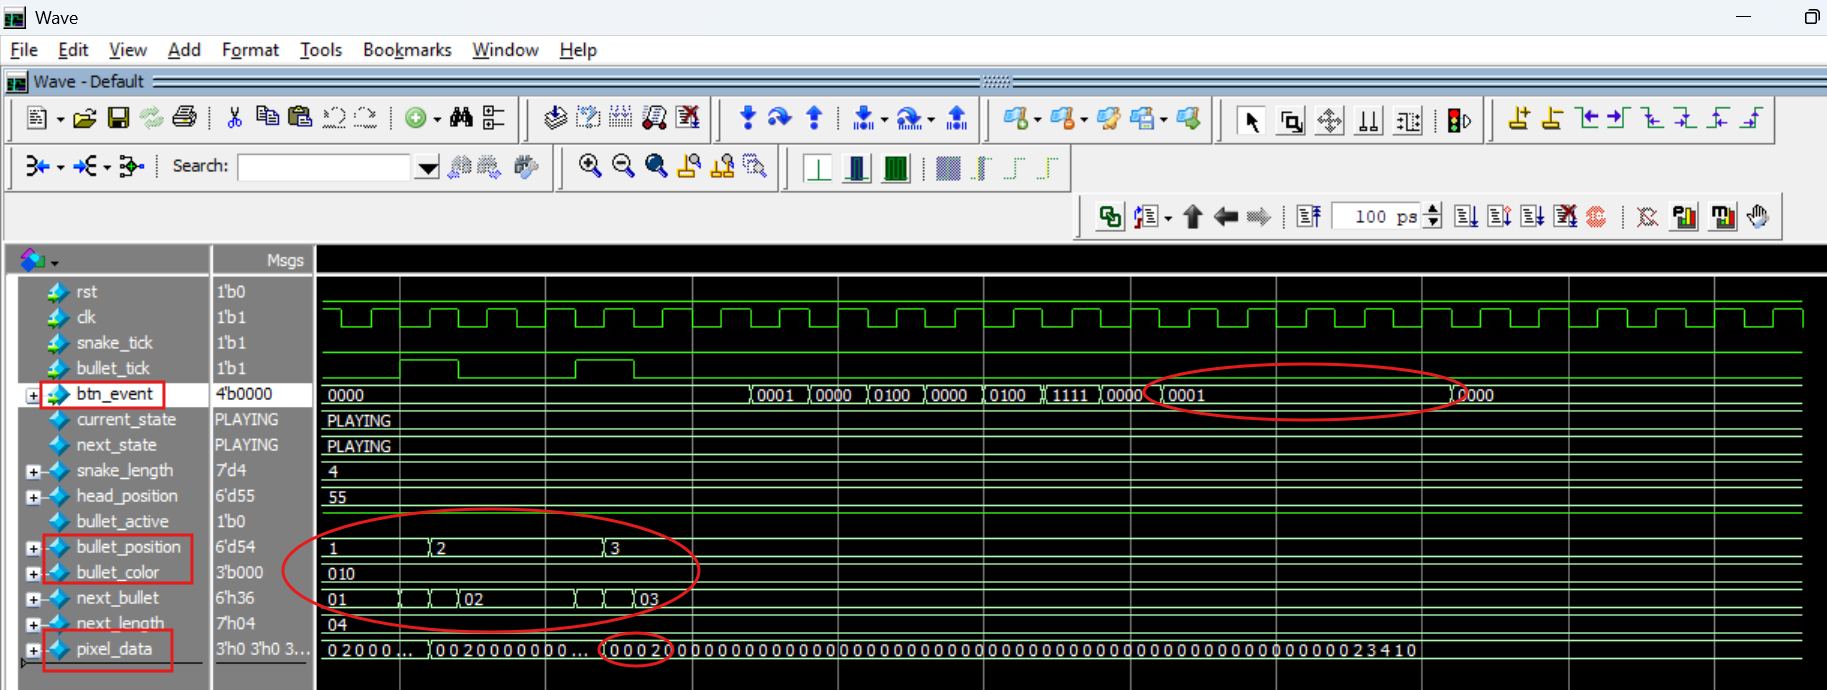
\includegraphics[width=0.95\textwidth]{images/game_engine_tc12_hold_zero.png}
    \caption{Dạng sóng kiểm tra giữ đè phím và xác nhận không sinh đạn đè tại LED 0}
    \label{fig:game-tc12-hold}
\end{figure}

\newpage

\section{Kết quả Mô phỏng Tích hợp Toàn hệ thống (Top-Level Verification)}

\subsection{Mục tiêu Kiểm thử}
Kiểm tra khả năng tích hợp toàn diện giữa các khối chức năng (\texttt{button\_conditioner}, \texttt{tick\_generator}, \texttt{game\_engine}, và \texttt{ws2812b\_driver}) trên module đỉnh \texttt{top\_snake\_game}. 

Mục tiêu chính bao gồm:
\begin{itemize}
    \item Xác minh tính đồng bộ của tín hiệu reset toàn hệ thống từ ngõ vào \texttt{rst\_sw}.
    \item Đảm bảo đường truyền điều khiển xuyên suốt: từ sự kiện nhấn phím vật lý (\texttt{key[3:0]}), qua bộ lọc xung, kích hoạt tạo đạn trên \texttt{game\_engine}, cập nhật mảng \texttt{pixel\_data} và truyền ra chân vật lý \texttt{led\_data\_out}.
    \item Xác minh khả năng bắt nhịp tự động giữa bộ tạo thời gian \texttt{tick\_generator} và logic di chuyển của trò chơi.
    \item Đảm bảo giao thức vật lý đơn dây 1-wire tại chân \texttt{led\_data\_out} tuân thủ chặt chẽ định thời bit chuẩn WS2812B thông qua việc đo đạc thời gian thực và giám sát liên tục bằng SystemVerilog Assertions (SVA).
\end{itemize}

\subsection{Quy trình Kiểm thử Đầu-cuối (End-to-End Verification Flow)}
Để tối ưu thời gian mô phỏng mà vẫn giữ nguyên bản chất hoạt động của mạch, testbench ghi đè các tham số phần cứng: \texttt{BULLET\_CYCLES = 20} chu kỳ clock (thay vì 2.500.000 chu kỳ), \texttt{RES = 40} chu kỳ (thay vì 15.000 chu kỳ), và kiểm thử trên quy mô rút gọn \texttt{LED\_COUNT = 6}.

Quy trình kiểm thử đầu-cuối thực thi tuần tự qua các giai đoạn:
\begin{enumerate}
    \item \textbf{Khởi tạo và Reset toàn hệ thống (TC1):} Kích hoạt xung \texttt{rst\_sw = 1}. Toàn bộ các module con được giám sát để xác nhận FSM chuyển về trạng thái ban đầu (\texttt{game\_engine} về \texttt{IDLE}, \texttt{ws2812b\_driver} về \texttt{LOAD}).
    \item \textbf{Chuyển trạng thái Vận hành (TC2):} Nhấn phím \texttt{key[2]} (active-low) để đưa toàn hệ thống từ \texttt{IDLE} sang \texttt{PLAYING}.
    \item \textbf{Luồng sự kiện xuyên suốt (TC3 \& TC4):} Nhấn \texttt{key[0]} để phát đạn RED. Testbench giám sát chuỗi phản hồi từ \texttt{key[0]} $\rightarrow$ sinh xung \texttt{btn\_event[0]} $\rightarrow$ \texttt{game\_engine} bật cờ \texttt{bullet\_active = 1}, gán màu RED $\rightarrow$ mảng \texttt{pixel\_data[0]} nhận mã RED. Đồng thời kiểm tra đúng ánh xạ dây (wiring) cho các phím còn lại (\texttt{key[1]}, \texttt{key[3]}).
    \item \textbf{Đồng bộ nhịp Tick nội bộ (TC5):} Đợi qua chu kỳ \texttt{BULLET\_CYCLES\_TEST} xung nhịp mà không can thiệp từ testbench để xác nhận \texttt{tick\_generator} phát xung nhịp tự nhiên làm tăng tọa độ \texttt{bullet\_position}.
    \item \textbf{Đo kiểm dạng sóng ngõ ra thực tế (TC6):} Sử dụng task tự động \texttt{read\_pixel\_24bit} đóng vai trò như một bộ thu WS2812B ảo, đo trực tiếp thời gian mức cao $T_H$ và mức thấp $T_L$ của từng bit trên đường truyền \texttt{led\_data\_out}. Dữ liệu 24-bit GRB giải mã được kiểm tra khớp với mã màu RED chuẩn (\texttt{24'h00\_3F\_00}).
\end{enumerate}

\subsection{Bằng chứng Mô phỏng Dạng sóng (Waveform Evidence)}

\subsubsection{Hành vi Reset, Khởi động và Kích hoạt Đạn xuyên suốt}
\begin{itemize}
    \item \textbf{Điều kiện kích thích:} Tác động \texttt{rst\_sw = 1}, sau đó lần lượt nhấn xung \texttt{key[2]} để vào \texttt{PLAYING} và nhấn \texttt{key[0]} để bắn đạn RED.
    \item \textbf{Kết quả mô phỏng:}
    \begin{itemize}
        \item Toàn bộ FSM của hệ thống được tái lập đồng bộ về trạng thái mặc định.
        \item Sườn xuống của \texttt{key[0]} được bộ lọc bắt chính xác và sinh ra đúng 1 xung \texttt{btn\_event[0]} tại sườn lên xung nhịp kế tiếp (thỏa mãn SVA \texttt{p\_btn0\_event}).
        \item Cờ \texttt{bullet\_active} bật lên 1 và \texttt{pixel\_data[0]} nạp thành công mã màu RED, chứng minh kết nối liên module thông suốt.
    \end{itemize}
\end{itemize}

\begin{figure}[H]
    \centering
    % \includegraphics[width=0.95\textwidth]{images/top_waveform_reset_and_fire.png}
    \caption{Dạng sóng kiểm tra Reset, chuyển trạng thái PLAYING và đường truyền nút nhấn xuyên suốt hệ thống}
    \label{fig:top_reset_fire}
\end{figure}

\subsubsection{Tịnh tiến Tự động và Kiểm tra Giao thức PWM tại led\_data\_out}
\begin{itemize}
    \item \textbf{Điều kiện kích thích:} Để mạch tự chạy dưới sự điều phối của \texttt{tick\_generator} và thu nhận chuỗi xung bit nối tiếp tại chân \texttt{led\_data\_out}.
    \item \textbf{Kết quả mô phỏng:}
    \begin{itemize}
        \item Xung \texttt{bullet\_tick} từ \texttt{tick\_generator} kích hoạt đúng chu kỳ, làm đạn tịnh tiến tự động sang vị trí kế tiếp mà không cần can thiệp ngoại vi.
        \item Tín hiệu nối tiếp trên chân \texttt{led\_data\_out} chuyển đổi trạng thái liên tục, không xuất hiện trạng thái treo mức cao quá 45 chu kỳ xung nhịp (thỏa mãn SVA \texttt{p\_no\_stuck\_high}).
        \item Dạng sóng PWM đạt đúng các thông số: Bit 0 ($T_H \approx 300\text{ ns}, T_L \approx 800\text{ ns}$) và Bit 1 ($T_H \approx 800\text{ ns}, T_L \approx 300\text{ ns}$), giải mã thành công 24-bit GRB của Pixel 0.
    \end{itemize}
\end{itemize}

\begin{figure}[H]
    \centering
    % \includegraphics[width=0.95\textwidth]{images/top_waveform_tick_and_pwm.png}
    \caption{Dạng sóng tịnh tiến đạn theo xung tick nội bộ và chuỗi xung PWM thực tế tại chân led\_data\_out}
    \label{fig:top_pwm}
\end{figure}

\newpage
\section{Tổng kết Kết quả Kiểm thử}

\subsection{Tổng hợp Kết quả Kiểm thử}

\begin{table}[H]
\centering
\caption{Tổng hợp kết quả kiểm thử các khối chức năng trong toàn bộ hệ thống}
\label{tab:system_test_summary}
\vspace{2mm}
\renewcommand{\arraystretch}{1.25}
\begin{tabularx}{\textwidth}{|l|X|c|c|}
\hline
\textbf{Khối chức năng} & \textbf{Phạm vi kiểm thử (Verification Scope)} & \textbf{Số TC} & \textbf{Kết quả} \\ \hline
\texttt{ws2812b\_driver} & FSM, tuần tự hóa dữ liệu, định thời xung PWM, chu kỳ chốt Latch, cô lập khung hình & 7 & \textbf{PASS} \\ \hline
\texttt{game\_engine} & FSM, động học rắn/đạn, phân giải va chạm, điều kiện WIN/LOSE, look-ahead anti-tunneling, chống spam phím & 12 & \textbf{PASS} \\ \hline
\texttt{button\_conditioner} & Đồng bộ xung nhịp, chống rung cơ học (debounce), bắt cạnh xung & --- & \textit{Not included} \\ \hline
\texttt{tick\_generator} & Phân tần số, tạo xung enable đơn chu kỳ 50 ms và 250 ms & --- & \textit{Not included} \\ \hline
\texttt{top\_snake\_game} & Tích hợp liên module, kết nối tín hiệu điều khiển và bus dữ liệu toàn hệ thống & 1 & \textbf{PASS} \\ \hline
\end{tabularx}
\end{table}

\subsection{Nhận xét Đánh giá}
Dựa trên kết quả mô phỏng chức năng trên môi trường QuestaSim, toàn bộ các khối xử lý trung tâm và ngoại vi giao tiếp của hệ thống đều đáp ứng đầy đủ các tiêu chuẩn kỹ thuật đề ra trong tài liệu đặc tả:
\begin{itemize}
    \item Khối \texttt{ws2812b\_driver} đã được chứng minh đáp ứng chặt chẽ các yêu cầu vật lý khắt khe về định thời xung số NZR, thực thi đúng quy trình tuần tự hóa dữ liệu MSB-first và bảo vệ toàn vẹn khung hình đang phát nhờ cơ chế chốt snapshot độc lập.
    \item Khối \texttt{game\_engine} thể hiện khả năng điều phối chính xác máy trạng thái FSM, tính toán động lực học di chuyển mượt mà theo từng nhịp tick, xử lý linh hoạt và chính xác các va chạm logic bằng kỹ thuật look-ahead mà không gặp hiện tượng tranh chấp hay xuyên đạn, đồng thời bảo đảm tính toàn vẹn của dữ liệu hiển thị \texttt{pixel\_data}.
\end{itemize}

\section{Kết luận và Hướng Phát triển}

\subsection{Những Kết quả Đạt được}
Đề tài đã hoàn thành các mục tiêu đề ra trong giai đoạn thiết kế và kiểm thử hệ thống phần cứng:
\begin{itemize}
    \item Hoàn thiện kiến trúc vi mạch số theo chuẩn thiết kế đồng bộ đơn miền xung nhịp 50 MHz sử dụng ngôn ngữ SystemVerilog.
    \item Hiện thực hóa đầy đủ các khối chức năng theo cấu trúc phân tầng rõ ràng giữa khối điều khiển (Control Flow) và đường dẫn dữ liệu (Data Path).
    \item Xây dựng môi trường kiểm thử tự động (Self-checking Testbench) với các task kích thích và assertion kiểm tra độc lập cho từng module.
    \item Xác minh thành công các hành vi chức năng trọng yếu và các trường hợp biên nguy hiểm thông qua phân tích dạng sóng mô phỏng chi tiết.
    \item Đóng gói và tích hợp thành công mô hình toàn hệ thống ở mức Top-level.
\end{itemize}

\subsection{Giới hạn của Báo cáo Kiểm thử}
Bên cạnh các kết quả đạt được, báo cáo kiểm thử này có một số giới hạn phạm vi như sau:
\begin{itemize}
    \item Các module \texttt{button\_conditioner} và \texttt{tick\_generator} không được trình bày dưới dạng chương mục báo cáo chi tiết riêng biệt do quy mô logic tương đối đơn giản và mang tính chất mạch đếm kinh điển; các module này đã được kiểm tra qua mô phỏng chức năng cơ bản trước khi tích hợp vào khối Top.
    \item Toàn bộ các kiểm thử mới dừng lại ở mức mô phỏng trước tổng hợp (Pre-synthesis Functional Simulation / RTL Simulation), chưa bao gồm kiểm thử trễ định thời thực tế (Gate-level / Post-fit Simulation with SDF timing back-annotation).
\end{itemize}

\subsection{Hướng Phát triển Tiếp theo}
Để hoàn thiện hệ thống hướng tới triển khai sản phẩm thương mại hoặc các thiết kế vi mạch chuyên sâu hơn, đề tài có thể tiếp tục mở rộng theo các hướng:
\begin{itemize}
    \item Mở rộng bộ Testbench tự động sang mô hình hướng đối tượng với phương pháp luận UVM (Universal Verification Methodology), tích hợp thêm Function Coverage và Code Coverage để đo lường độ phủ kiểm thử.
    \item Bổ sung hệ thống SystemVerilog Assertions (SVA) tĩnh và động vào mã nguồn RTL để bắt lỗi giao tiếp bus và lỗi định thời ngay trong thời gian thực.
    \item Tiến hành nạp bitstream lên kit FPGA Altera DE2 vật lý (Cyclone II EP2C35F672C6), đo đạc dạng sóng thực tế trên chân GPIO bằng máy hiện sóng (Oscilloscope / Logic Analyzer) và đánh giá độ trễ nhiệt/định thời (Timing Closure).
\end{itemize}

\end{document}